\chapter{Response Measurement with Single Hadrons}

\label{ch:singlehadrons}
% --------------------------------------------------------------------------------

As discussed in Section~\ref{sec:jets}, colored particles produced in collisions hadronize into jets of multiple hadrons.
One approach to understanding jet energy measurements in the ATLAS calorimeters is to evaluate the calorimeter response to those individual hadrons; measurements of individual hadrons can be used to build up an understanding of the jets that they form.
The redundancy of the momentum provided by the tracking system and the energy provided by the calorimeter provides an opportunity to study calorimeter response using real collisions, as described further in Section~\ref{sec:inclusive}.

Calorimeter response includes a number of physical effects that can be extracted to provide insight into many aspects of jet modeling.
First, many charged hadrons interact with the material of the detector prior to reaching the calorimeters and thus do not deposit any energy.
Comparing this effect in data and simulation is a powerful tool in validating the interactions of particles with the material of the detector and the model of the detector geometry in simulation, see Section~\ref{sec:zero_fraction}.
The particles which do reach the calorimeter deposit their energy into several adjacent cells, which are then clustered together.
The energy of the cluster is then the total energy deposited by that particle.
Comparing the response of hadrons in data to that of simulated hadrons provides a direct evaluation of the showering of hadronic particles and the energy deposited by particles in matter (Section~\ref{sec:response}). 

The above studies all use an inclusive selection of charged particles, which are comprised predominantly of pions, kaons, and (anti)protons.
It is also possible to measure the response to various identified particle types separately to evaluate the simulated interactions of each particle, particularly at low energies where differences between species are very relevant.
Pions and (anti)protons can be identified through decays of long-lived particles, in particular $\Lambda$, $\overline{\Lambda}$, and $K_{S}^{0}$, and then used to measure response as described above.
This is discussed in detail in Section~\ref{sec:identified}.

The results in this chapter use data collected at 7 and 8 \TeV collected in 2010 and 2012, respectively.
Both are included as the calorimeter was repaired and recalibrated between those two data-taking periods.
Both sets of data are compared to an updated simulation that includes new physics models provided by \texttt{Geant4}~\cite{GEANT4} and improvements in the detector description~\cite{PERF-2011-08,PERF-2013-05}.
The present results are published in \ac{EPJC}~\cite{PERF-2015-05} and can be compared to a similar measurement performed in 2009 and 2010~\cite{PERF-2011-05}, which used the previous version of the simulation framework~\cite{SOFT-2010-01}.

% ----------------------------------------
\section{Dataset and Simulation}

\subsection{Data Samples}
The two datasets used in this chapter are taken from dedicated low-pileup runs where the fraction of events with multiple interactions was negligible.
These datasets are used rather than those containing full-pileup events to facilitate measurement of isolated hadrons.
The 2012 dataset at $\sqrt{s} = 8$ \TeV contains 8 million events and corresponds to an integrated luminosity of 0.1 nb\tsup{-1}.
The 2010 dataset at $\sqrt{s} = 7$ \TeV contains 3 million events and corresponds to an integrated luminosity of 3.2 nb\tsup{-1}.
The latter dataset was also used for the 2010 results~\cite{PERF-2011-05}, but it has since been reanalyzed with an updated reconstruction including the final, best understanding of the detector description for the material and alignment from Run 1.

\subsection{Simulated Samples}
The two datasets above are compared to simulated single-, double-, and non-diffractive events generated with \texttt{Pythia8}~\cite{PYTHIA8} using the A2 configuration of hadronization~\cite{AU2} and the MSTW 2008 parton-distribution function set~\cite{MSTW,MSTW2}.
The admixture of the single-, double-, and non-diffractive events uses the default relative contributions from \texttt{Pythia8}.
The conditions and energies for the two simulations are chosen so that they match those of the corresponding dataset.

To evaluate the interaction of hadrons with detector material, the simulation uses two different collections of hadronic physics models, called physics lists, in \texttt{Geant4 9.4}~\cite{G4hadronics}.
The first, \QGSP, combines the Bertini intra-nuclear cascade~\cite{BERT21,BERT22,BERT23} below 9.9 \GeV, a parametrized proton inelastic model from 9.5 to 25 \GeV~\cite{GHEISHA20}, and a quark-gluon string model above 12 \GeV~\cite{QGS15,QGS16,QGS17,QGS18,QGS19}. 
The second, \FTFP, combines the Bertini intra-nuclear cascade~\cite{BERT21,BERT22,BERT23} below 5 \GeV and the Fritiof model~\cite{FTF24,FTF25,FTF26,FTF27} above 4 \GeV.
In either list, \texttt{Geant4} enforces a smooth transition between models where multiple models overlap.

\subsection{Event Selection}
\label{sec:inclusive_selection}
The event selection for this study is minimal, as the only requirement is selecting good-quality events with an isolated track. 
Such events are triggered by requiring at least two hits in the minimum-bias trigger scintillators. 
After trigger, each event is required to have exactly one reconstructed vertex, and that vertex is required to have four or more associated tracks.

The particles which are selected for the response measurements are first identified as tracks in the inner detector.
The tracks are required to have at least 500 \MeV of transverse momentum.
To ensure a reliable momentum measurement, these tracks are required to have at least one hit in the pixel detector, six hits in the SCT, and small longitudinal and transverse impact parameters with respect to the primary vertex~\cite{PERF-2011-05}.
For the majority of the measurements in this chapter, the track is additionally required to have 20 hits in the TRT, which significantly reduces the contribution from tracks which undergo nuclear interactions.
This requirement and its effect is discussed in more detail in Section~\ref{sec:additional}. 
In addition, tracks are rejected if there is any other reconstructed track which extrapolates to the calorimeter within a cone of $\Delta R = \sqrt{(\Delta\phi)^2 + (\Delta\eta)^2} < 0.4$.
This requirement guarantees that the contamination of energy from nearby charged particles is negligible~\cite{PERF-2011-05}.

% ----------------------------------------

\section{Inclusive Hadron Response}
\label{sec:inclusive}

The calorimeter response is more precisely defined as the ratio of the measured calorimeter energy to the true energy carried by the particle, although this true energy is unknown. 
For charged particles, however, the inner detector provides a very precise measurement of momentum (with uncertainty less than 1\%) that can be used as a proxy for true energy.
The ratio of the energy deposited by the charged particle in the calorimeter, $E$, to its momentum measured in the inner detector $p$, forms the calorimeter response measure called \ep.
Though the distribution of \ep contains a number of physical features, this study focuses on the trends in two aggregated quantities: \epav, the average of \ep for the selected tracks, and the zero fraction, the fraction of tracks with no associated energy in the calorimeter for those tracks.

The calorimeter energy assigned to a track is defined using clusters. 
The clusters are formed using a 4--2--0 algorithm~\cite{TopoClusters} that begins with seeds requiring at least 4 times the average calorimeter cell noise. 
The neighboring cells with at least twice that noise threshold are then added to the cluster, and all bounding cells are then added with no requirement. 
This algorithm minimizes noise contributions through its seeding process, and including the bounding cells improves the energy resolution~\cite{Speckmayer}.
The clusters are associated to a given track if they fall within a cone of $\Delta R = 0.2$ of the extrapolated position of the track, which includes about 90\% of the energy on average~\cite{PERF-2011-05}.

\subsection{E/p Distribution}

The \ep distributions measured in both data and simulation are shown in Figure~\ref{fig:eoverp} for two example bins of track momentum and for tracks in the central region of the detector. 
These distributions show several important features of the \ep observable.
The large content in the bin at $E=0$ comes from tracks that have no associated cluster, which occurs due to interactions with detector material prior to reaching the calorimeter or the energy deposit being insufficiently large to generate a seed, and are discussed in Section~\ref{sec:zero_fraction}.
The small negative tail also comes from tracks that do not deposit any energy in the calorimeter but are randomly associated to a cluster with an energy below the noise threshold.
The long positive tail above 1.0 comes from the contribution of neutral particles.
Nearby neutral particles deposit (sometimes large) additional energy in the calorimeter but do not produce tracks in the inner detector, so they cannot be rejected by the track isolation requirement.
Additionally the peak and mean of the distribution falls below 1.0 because of the loss of energy not found within the cone as well as the non-compensation of the calorimeter.

The data and simulation share the same features, but the high and low tails are significantly different.
The simulated events tend to overestimate the contribution of neutral particles to the long tail, an effect which can be isolated and removed as discussed in Section~\ref{sec:neutral_bg}. 
Additionally, the simulated clusters have less noise on average, although this is a small effect on the overall response.

\begin{figure}[htbp]
\centering
\subfloat[]{
  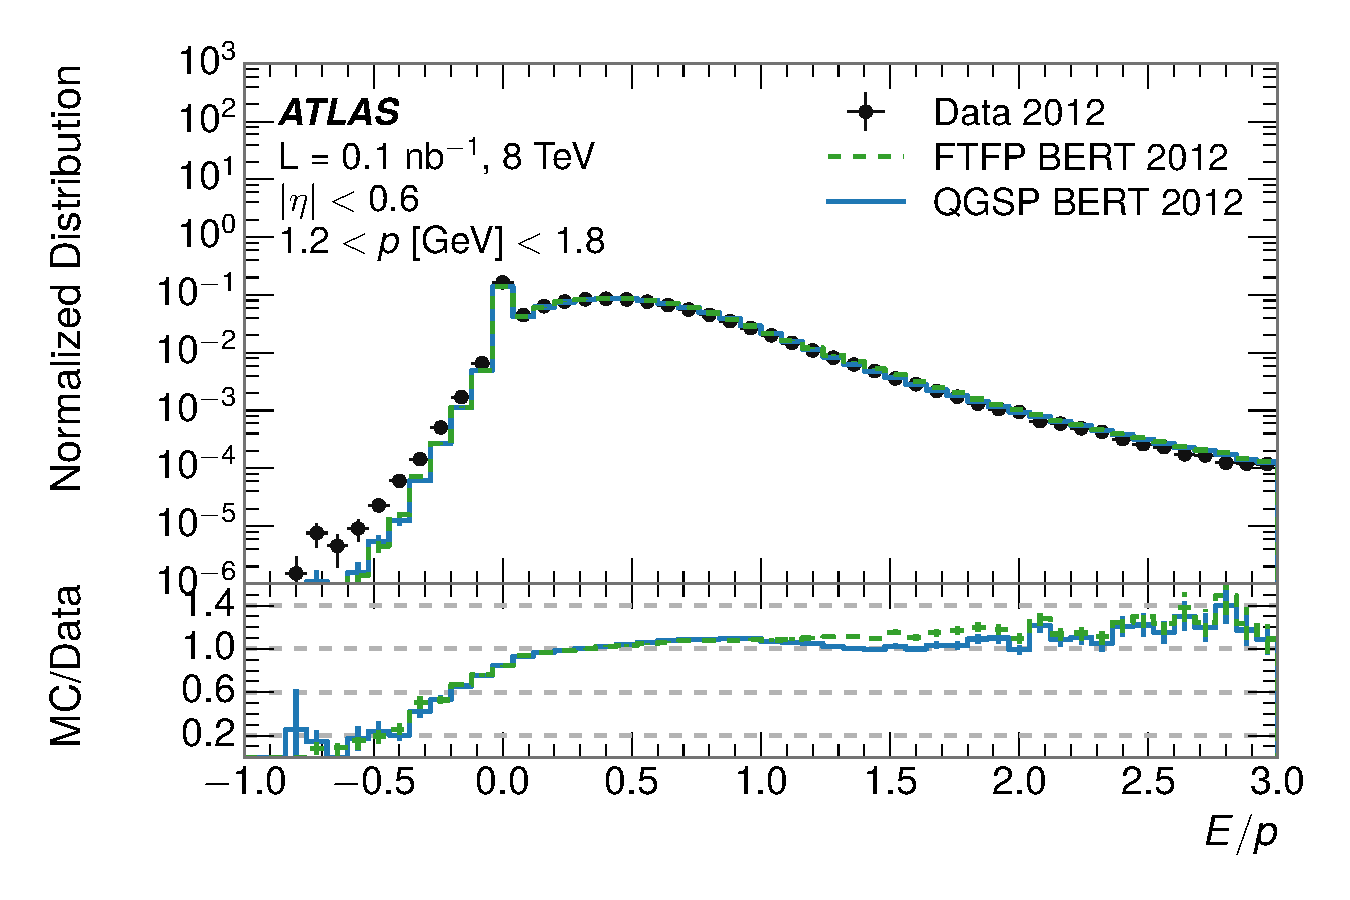
\includegraphics[width=\halffig]{figures/dvmc12_eoverp_layer01_calib01_eta01_p03_q00_nc00_trt00.pdf}
}
\subfloat[]{
  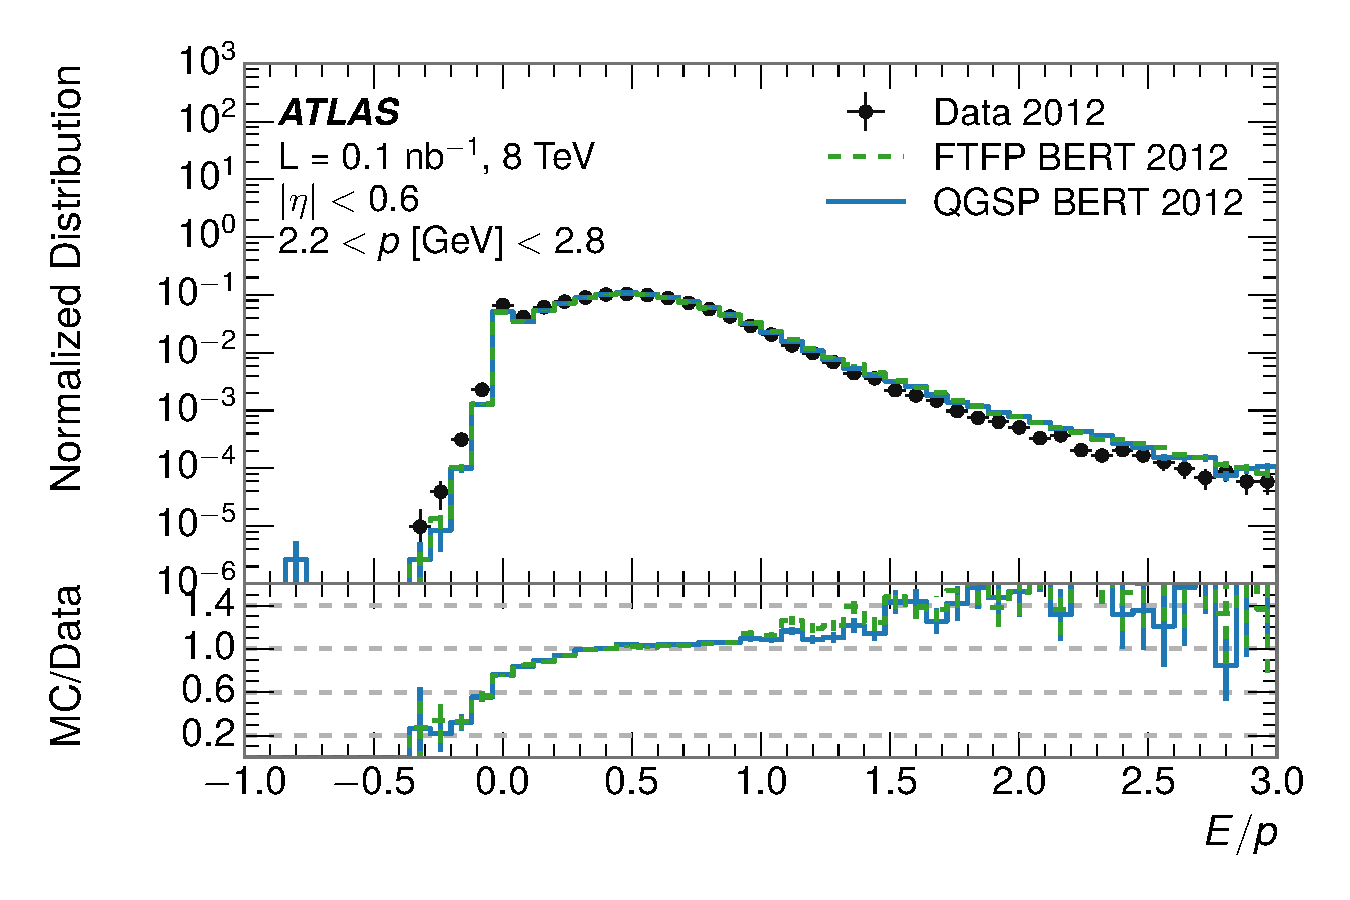
\includegraphics[width=\halffig]{figures/dvmc12_eoverp_layer01_calib01_eta01_p05_q00_nc00_trt00.pdf}
}
\caption{The \ep distribution and ratio of simulation to data for isolated tracks with (a) $|\eta| < 0.6$ and $1.2 < p /\GeV < 1.8$ and (b) $|\eta| < 0.6$ and $2.2 < p /\GeV < 2.8$.}

\label{fig:eoverp}
\end{figure}

\subsection{Zero Fraction}
\label{sec:zero_fraction}

The fraction of particles with no associated clusters, or similarly those with $E \leq 0$, reflects the modeling of both the detector geometry and hadronic interactions.
The zero fraction is expected to rise as the amount of material a particle traverses increases, while it is expected to decrease as the particle energy increases.
This dependence can be seen in Figure~\ref{fig:zerofracincl}, where the zero fraction in data and simulation is shown as a function of momentum and the amount of material measured in interaction lengths.
The trends are similar between 2010 and 2012 and for positively and negatively charged particles.
The zero fraction decreases with energy as expected.
The absolute discrepancy in zero fraction between data and simulation decreases with momentum from 5\% to less than 1\%, but this becomes more pronounced in the ratio as the zero fraction shrinks quickly with increasing momentum.
The amount of material in the detector increases with $\eta$, which is used to obtain results for interaction lengths ranging between 0.1 and 0.65~$\lambda$.
As the data and simulation have significant disagreement in the zero fraction over a number of interaction lengths, the difference must be primarily from the modeling of hadronic interactions with detector material and not just the detector geometry.
Although two different hadronic interaction models are shown in the figure, they have very similar discrepancies to data because both use the same description (the BERT model) at low momentum.

\begin{figure}[htbp]
\centering
\subfloat[]{
  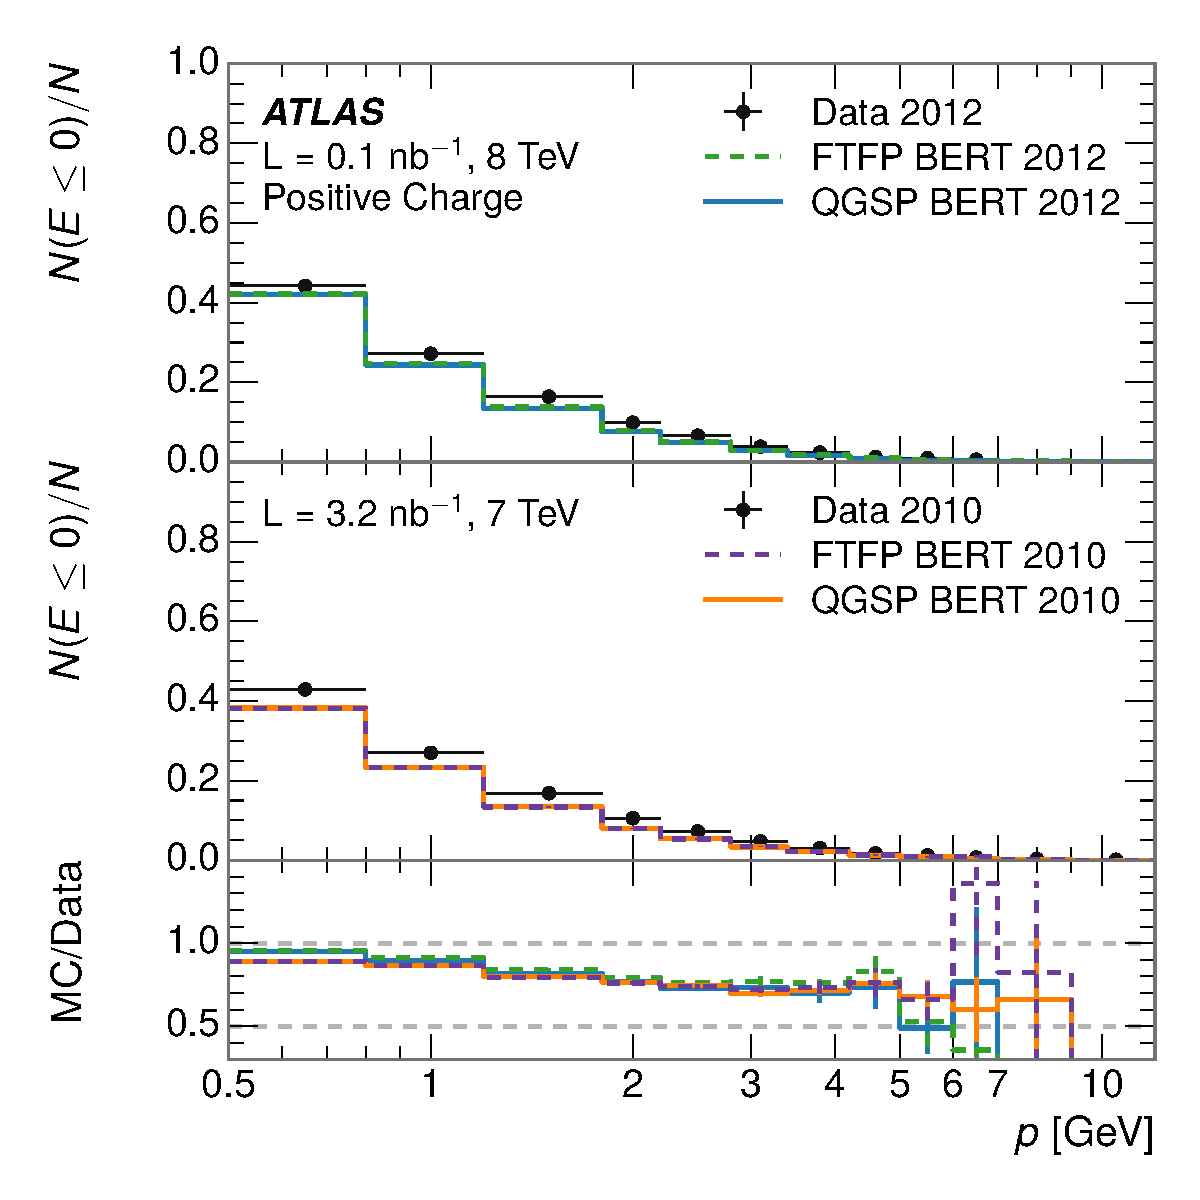
\includegraphics[width=\halffig]{figures/dvmc_ezero_layer01_calib01_eta01_q02_nc00_trt00.pdf}
}
~
\subfloat[]{
  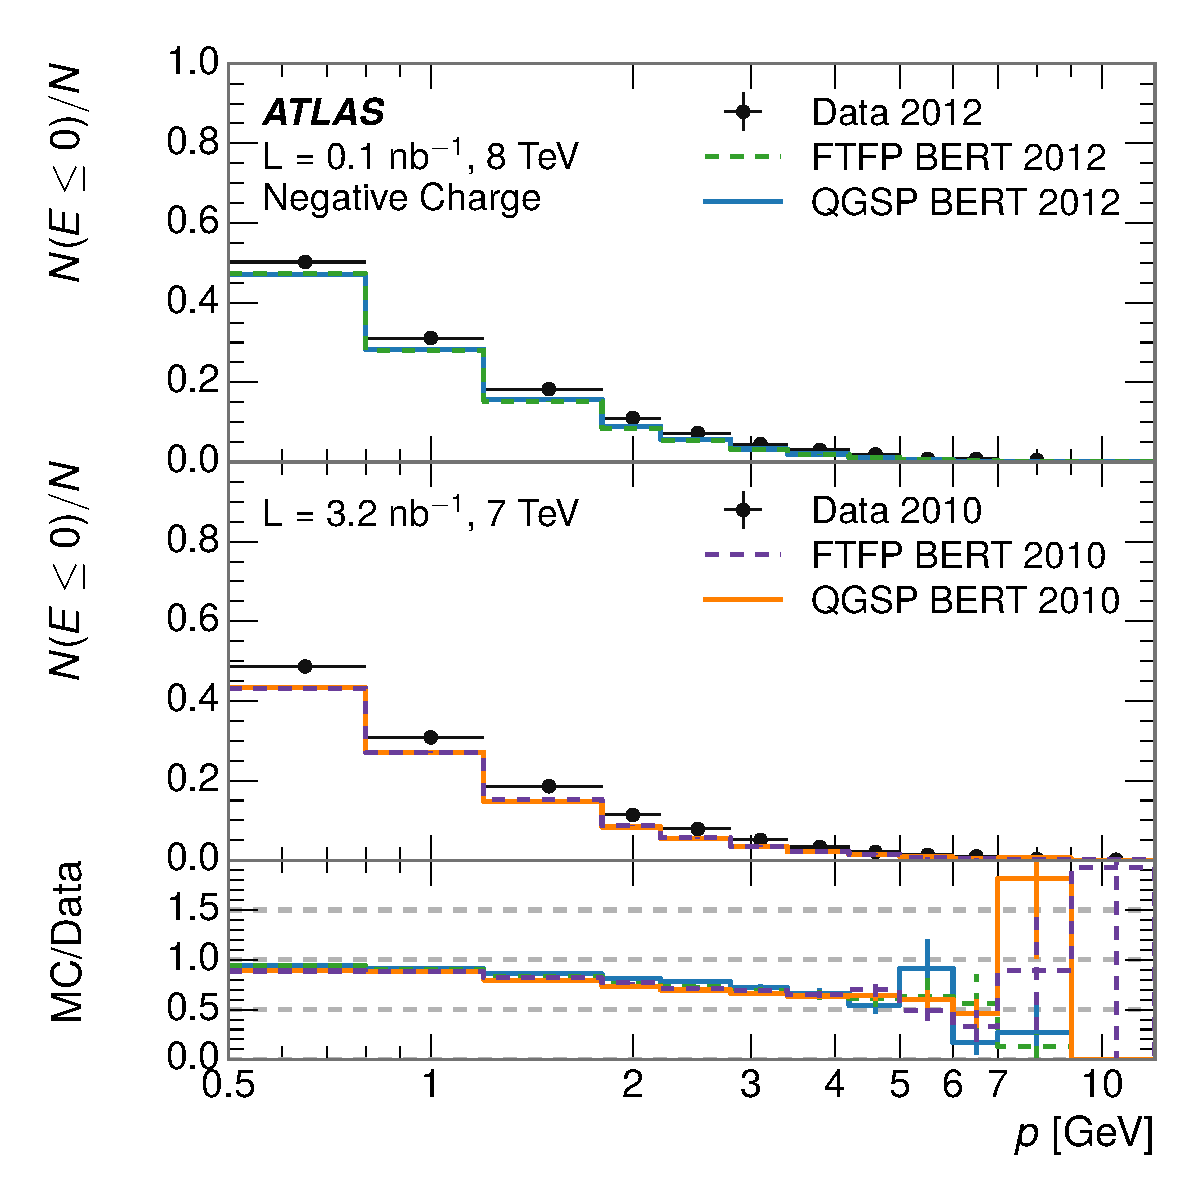
\includegraphics[width=\halffig]{figures/dvmc_ezero_layer01_calib01_eta01_q01_nc00_trt00.pdf}
}
\\
\subfloat[]{
  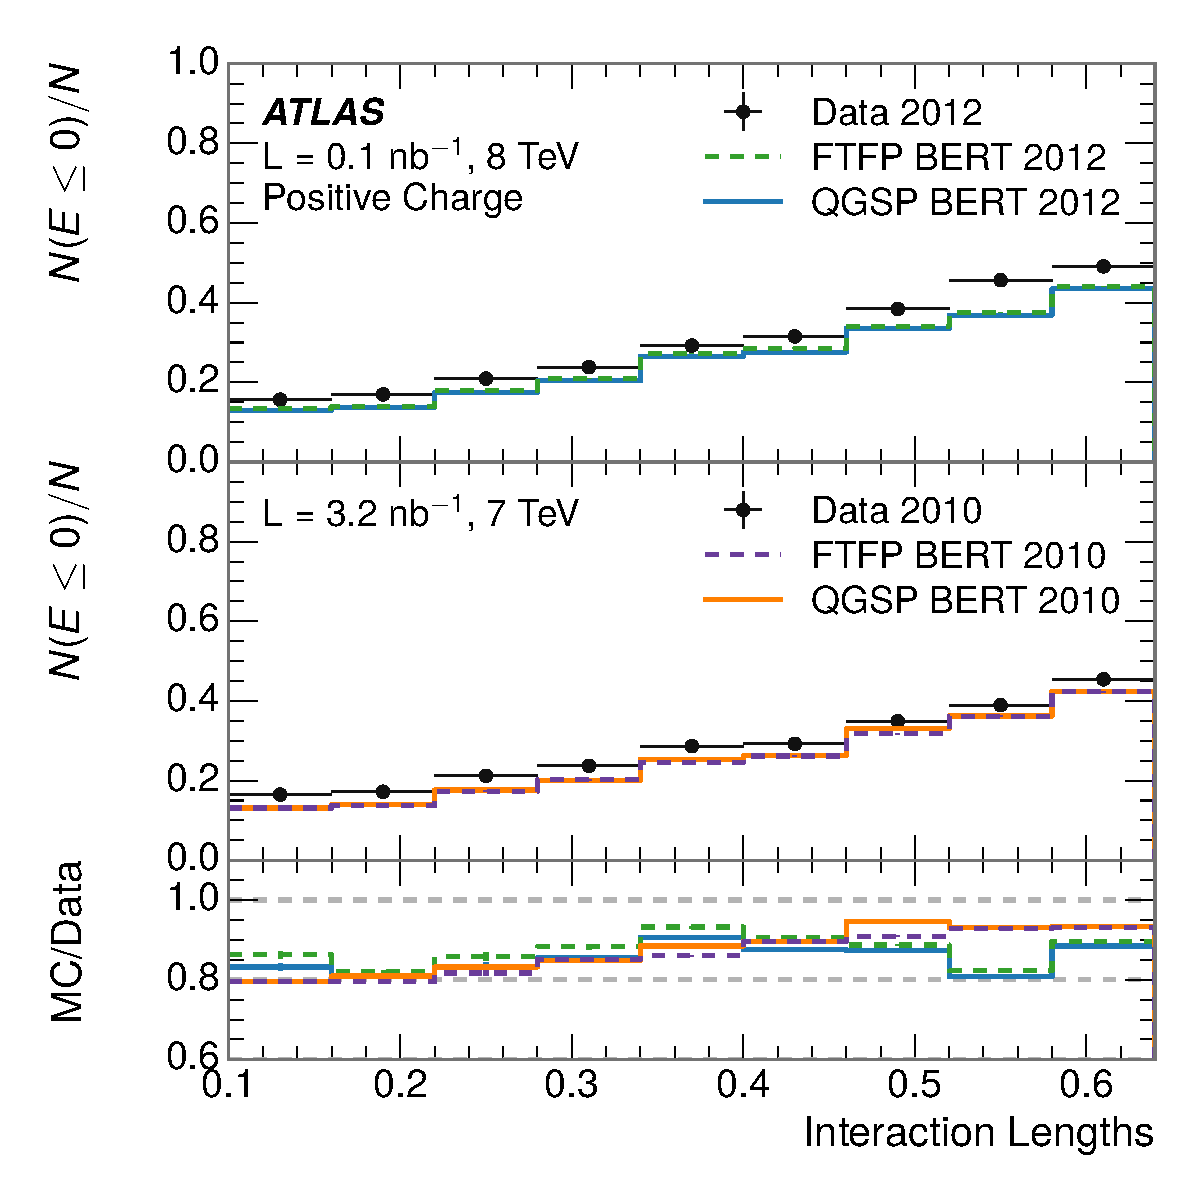
\includegraphics[width=\halffig]{figures/ezero_intlen_q02.pdf}
}
~
\subfloat[]{
  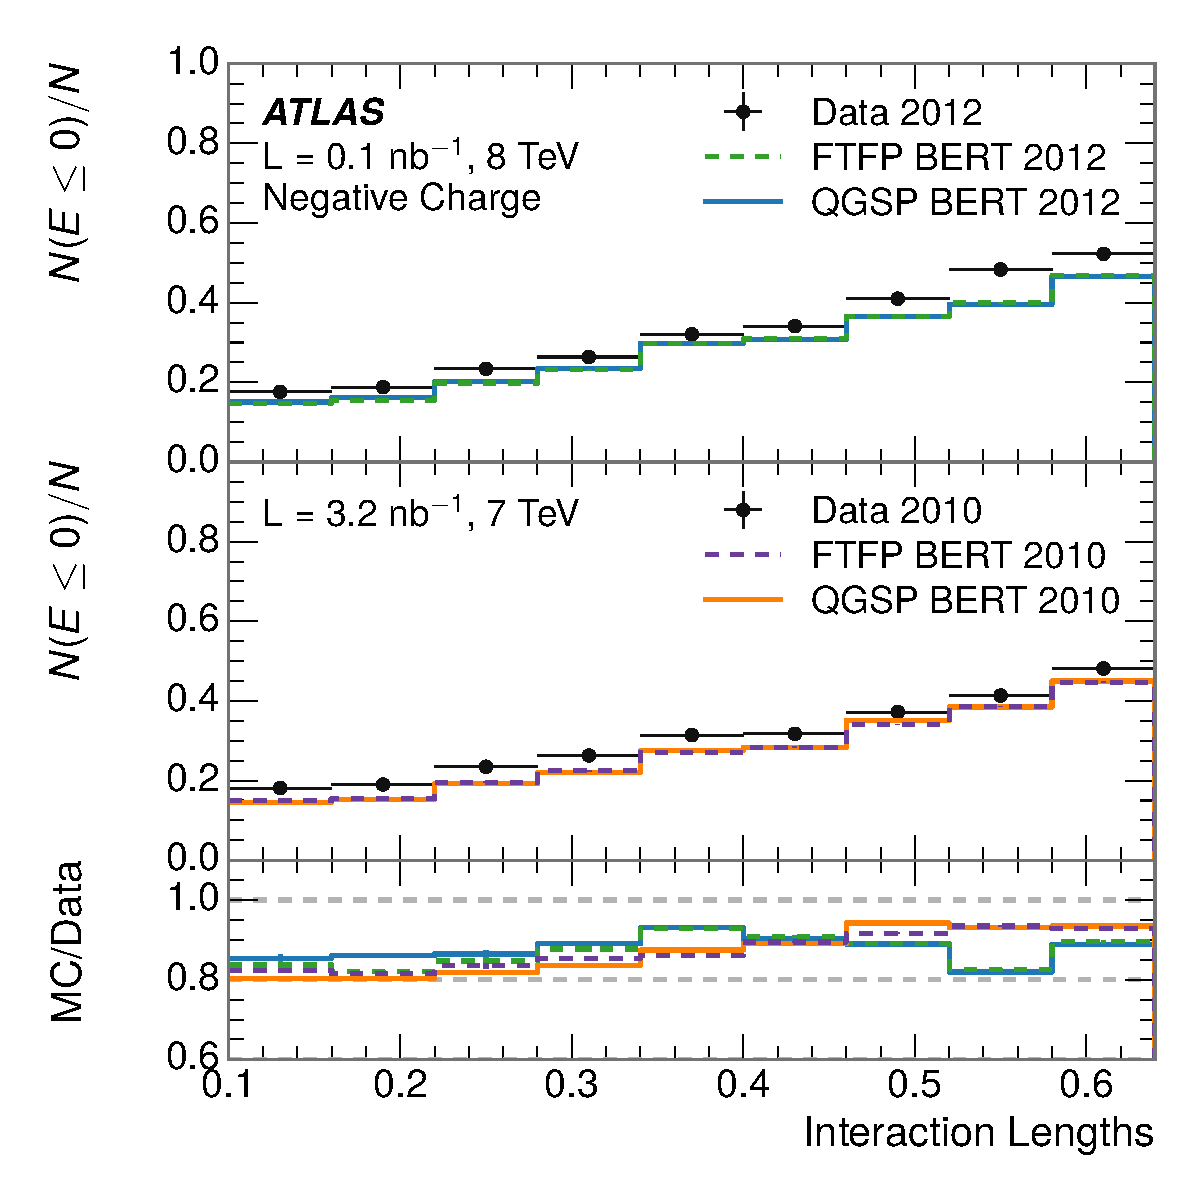
\includegraphics[width=\halffig]{figures/ezero_intlen_q01.pdf}
}
\caption{The fraction of tracks as a function (a, b) of momentum, (c, d) of interaction lengths with $E \leq 0$ for tracks with positive (on the left) and negative (on the right) charge.}
\label{fig:zerofracincl}
\end{figure}


\subsection{Neutral Background Subtraction}
\label{sec:neutral_bg}

The isolation requirement on hadrons is only effective in removing an energy contribution from nearby charged particles. 
Nearby neutral particles, predominantly photons from \piz decays, also add their energy to the calorimeter clusters, but mostly in the electromagnetic calorimeter. 
The arrangement of energy deposits is shown in Figure~\ref{fig:eoverp_cartoon}, which illustrates both energy deposits from the hadronic particle and additional deposits from neutral particles.
It is possible to measure this contribution, on average, using late-showering hadrons that minimally ionize in the electromagnetic calorimeter. 
Such particles are selected by requiring that they deposit less than 1.1 \GeV in the EM calorimeter within a cone of $\Delta R < 0.1$ around the track. 
To ensure that these particles are well measured, they are additionally required to deposit between 40\% and 90\% of their energy in the hadronic calorimeter within the same cone. 

\begin{figure}[htbp]
\centering
\subfloat[]{
  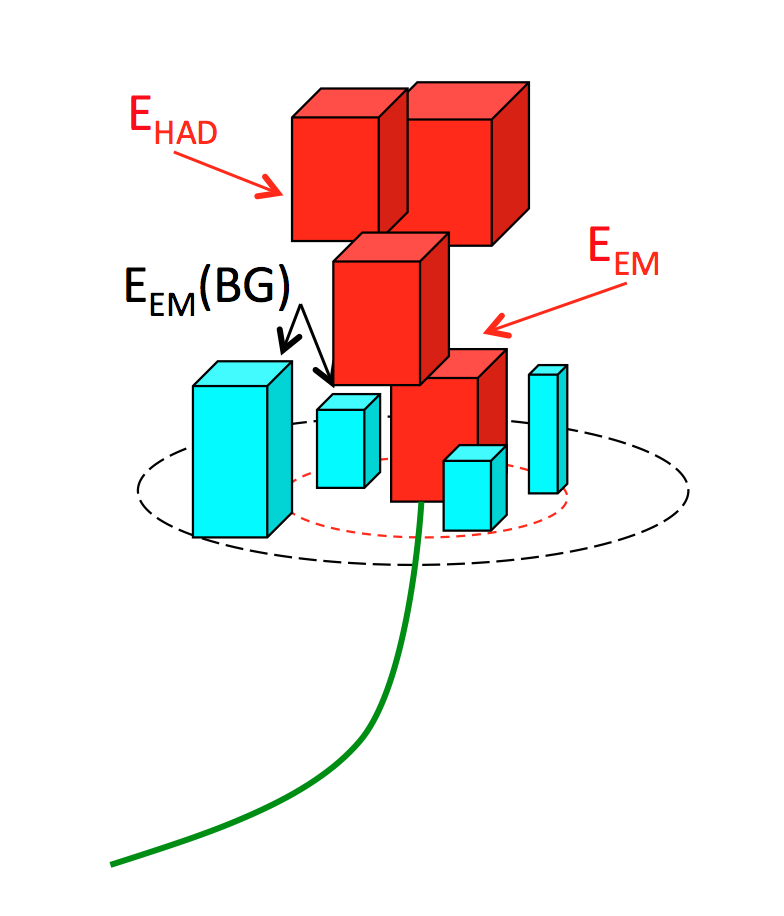
\includegraphics[width=.4\textwidth]{figures/SignalDiagram.png}
}
\subfloat[]{
  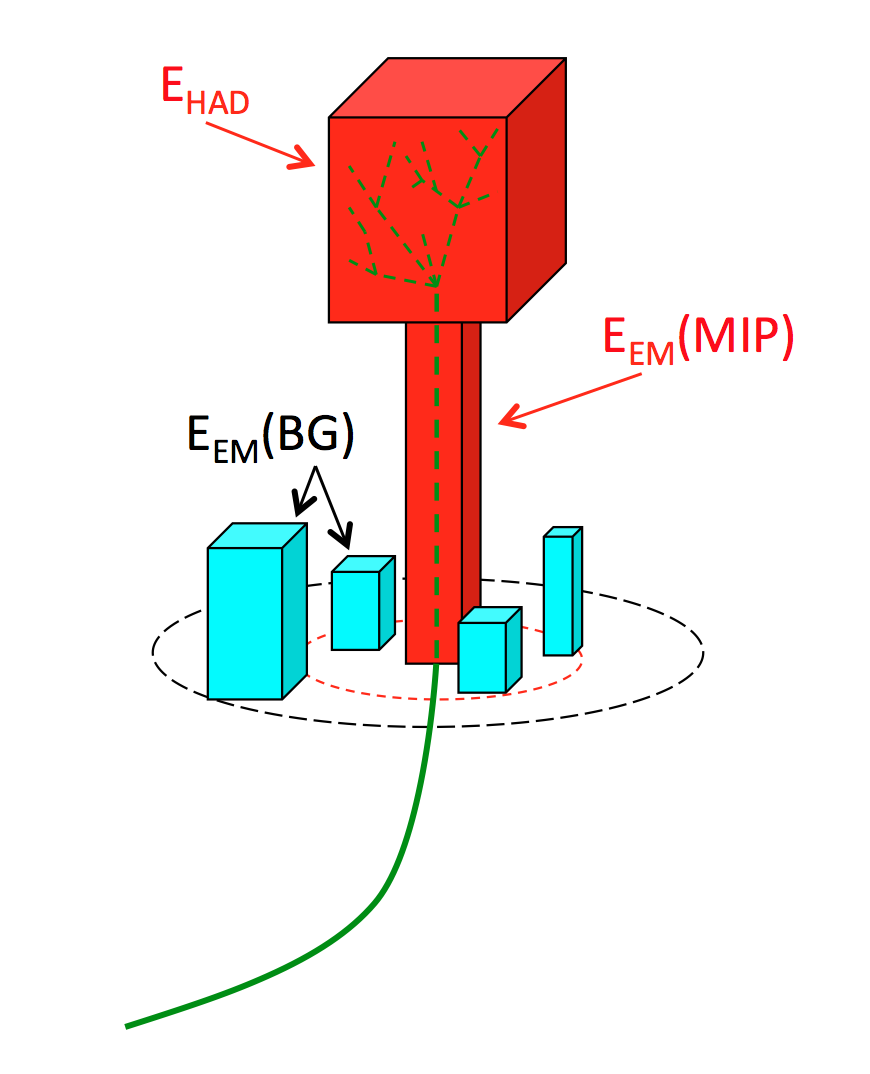
\includegraphics[width=.4\textwidth]{figures/BGDiagram.png}
}
\caption{An illustration (a) of the geometry of energy deposits in the calorimeter. The red energy deposits come from the charged particle targeted for measurement, while the blue energy deposits are from nearby neutral particles and must be subtracted. The same diagram (b) for the neutral-background selection, described in Section~\ref{sec:neutral_bg}.}
\label{fig:eoverp_cartoon}
\end{figure}

These particles provide a clean sample to measure the nearby neutral background because they do not deposit energy in the area immediately surrounding them in the EM calorimeter, as shown in Figure~\ref{fig:eoverp_cartoon}.
So, the energy deposits in the region $0.1 < \Delta R < 0.2$ can be attributed to neutral particles alone.
To estimate the contribution to the whole cone considered for the response measurement, that energy is scaled by a geometric factor of 4/3. 
This quantity, \epbg, measured in aggregate over a number of particles, gives the contribution to \epav from neutral particles in the EM calorimeter. 
Similar techniques were used in the individual layers of the hadronic calorimeters to show that the background from neutrals is negligible in those layers~\cite{PERF-2011-05}. 

The distribution of this background estimate is shown in Figure~\ref{fig:eoverp_background} for data and simulation with the two different physics lists.
The contribution from neutral particles falls from 0.1 at low momentum to around 0.03 for particles above 7 \GeV. 
Although the simulation captures the overall trend, it significantly overestimates the neutral contribution for tracks with momentum between 2 and 8 \GeV.
This effect was also seen in the tails of the \ep distributions in Figure~\ref{fig:eoverp}.
This difference is likely due to modeling of coherent neutral particle radiation in \texttt{Pythia8} that overestimates the production of \piz near the production of the charged particles.
The discrepancy does not depend on $\eta$ and thus is unlikely to be a mismodeling of the detector.
This difference can be subtracted to form a corrected average of \ep.

\begin{figure}[htbp]
\centering
\subfloat[]{
  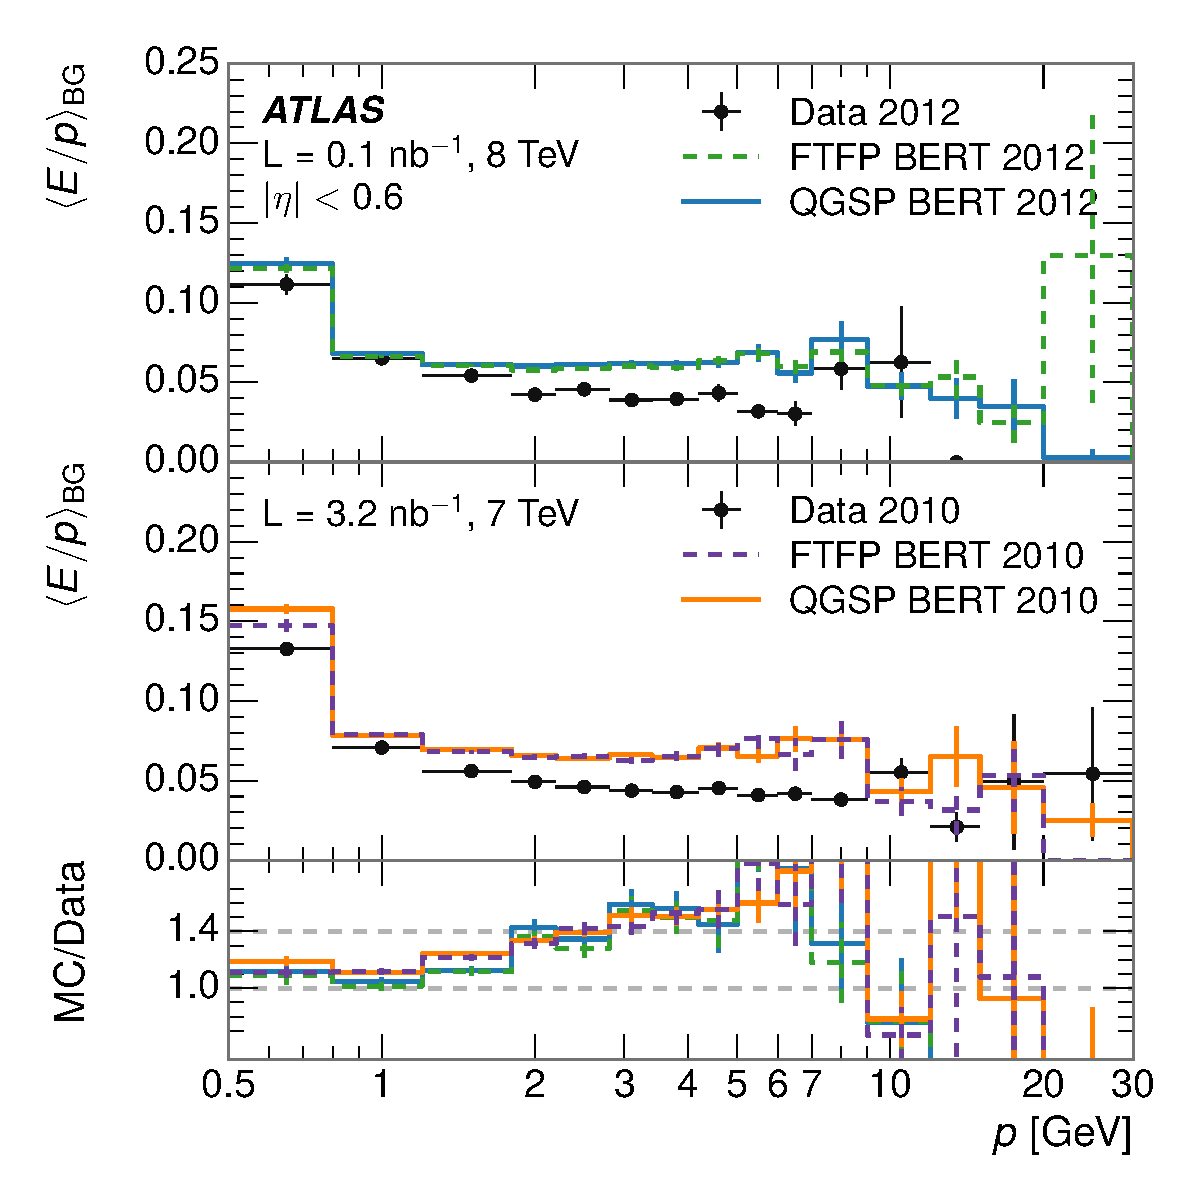
\includegraphics[width=\halffig]{figures/dvmc_epbg_layer01_calib01_eta01_q00_nc00_trt02.pdf}
}
~
\subfloat[]{
  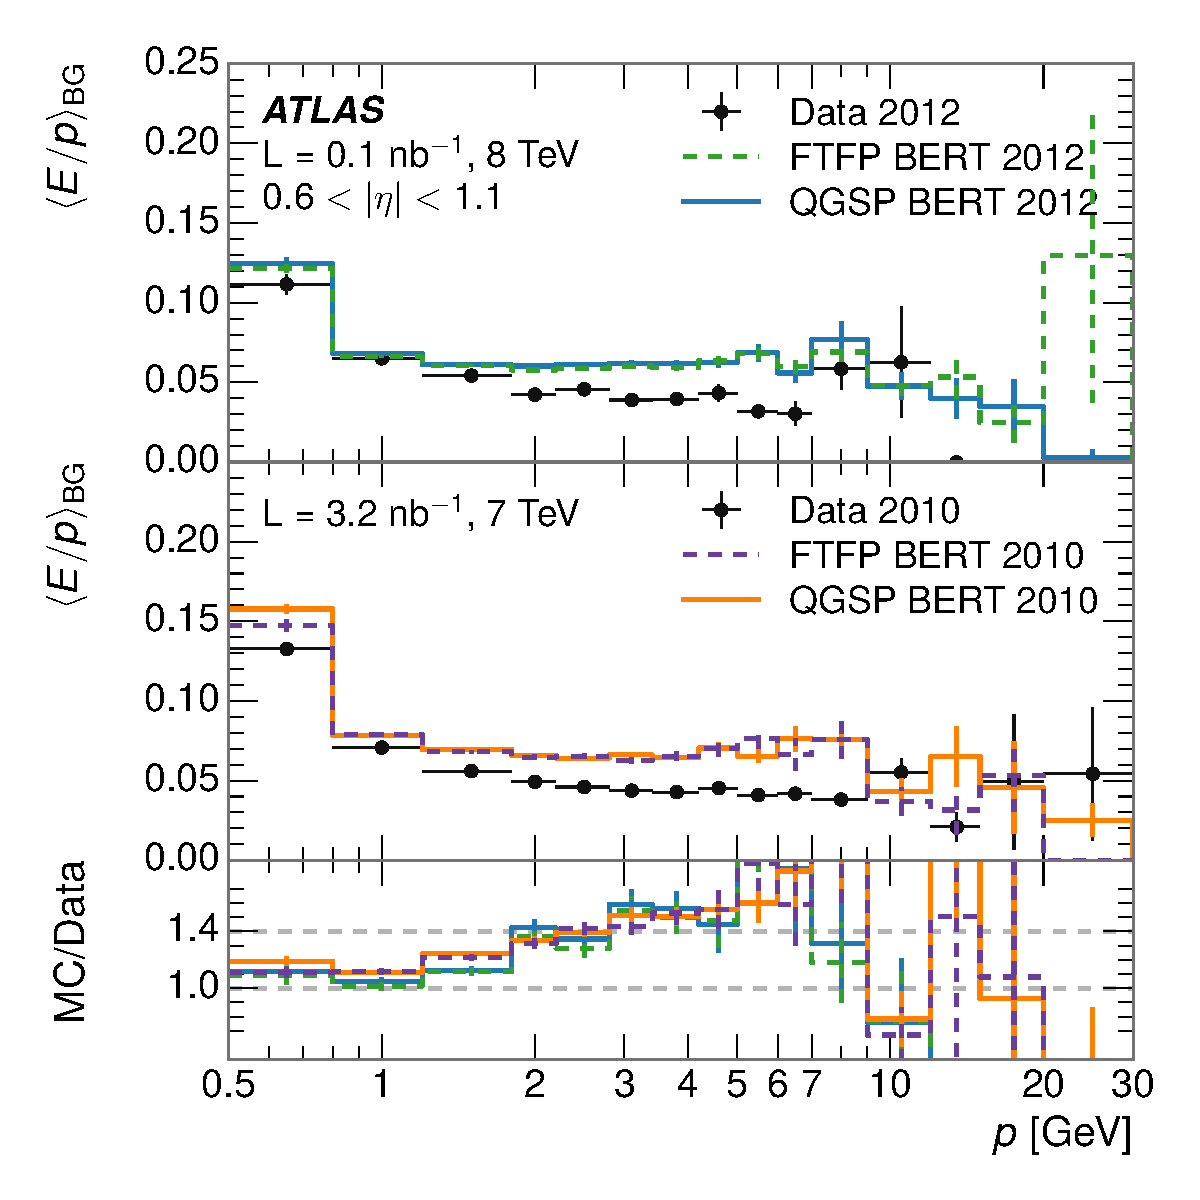
\includegraphics[width=\halffig]{figures/dvmc_epbg_layer01_calib01_eta02_q00_nc00_trt02.pdf}
}
\\
\subfloat[]{
  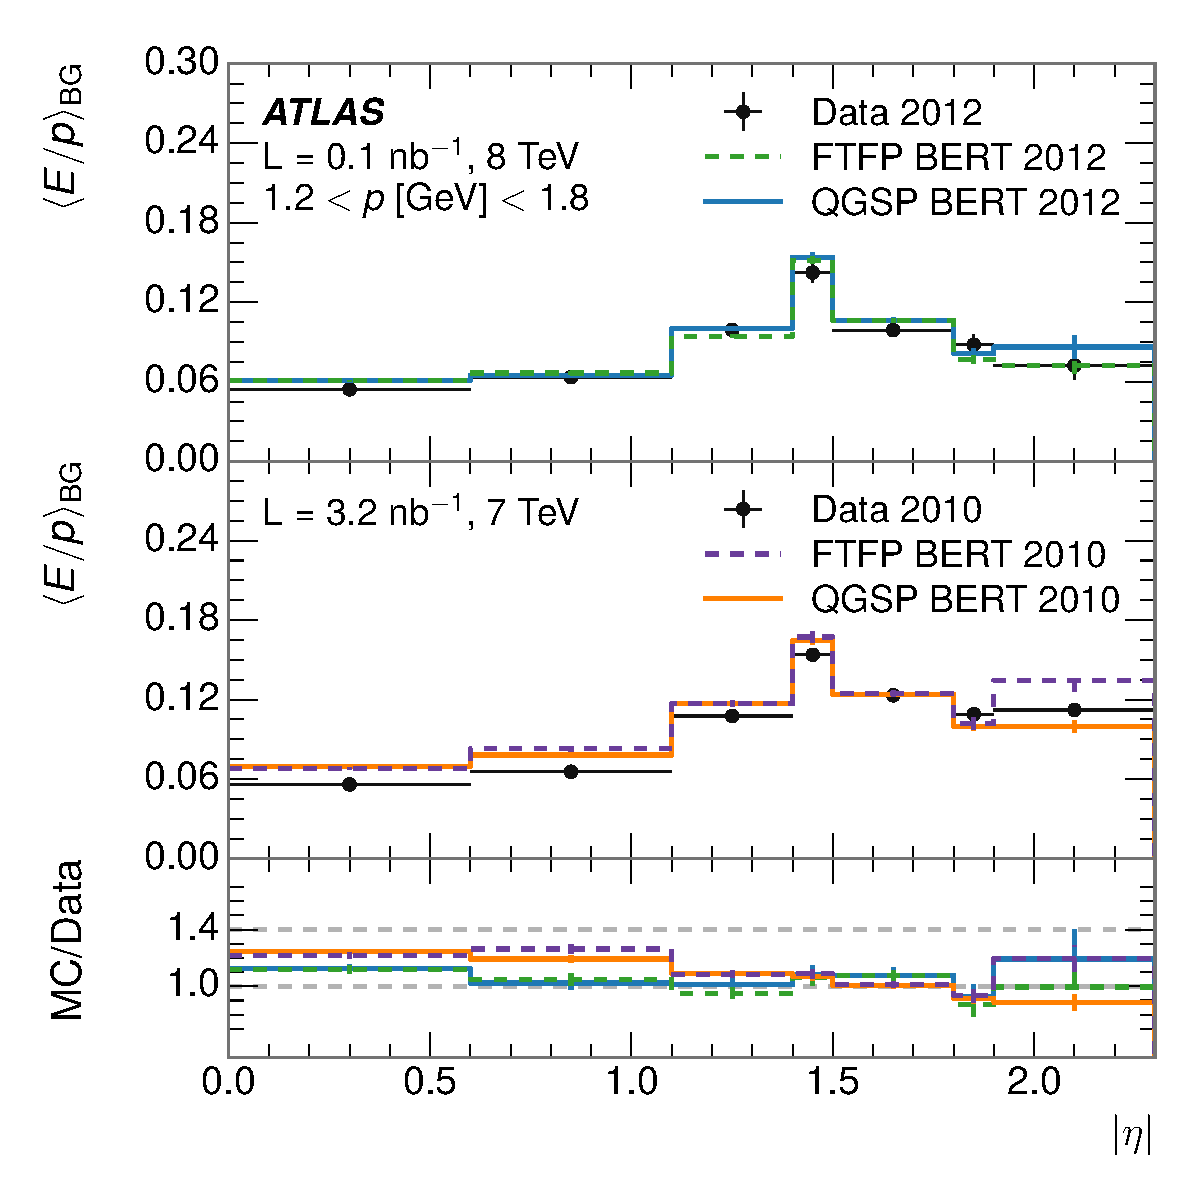
\includegraphics[width=\halffig]{figures/dvmc_epbg_layer01_calib01_p03_q00_nc00_trt02.pdf}
}
~
\subfloat[]{
  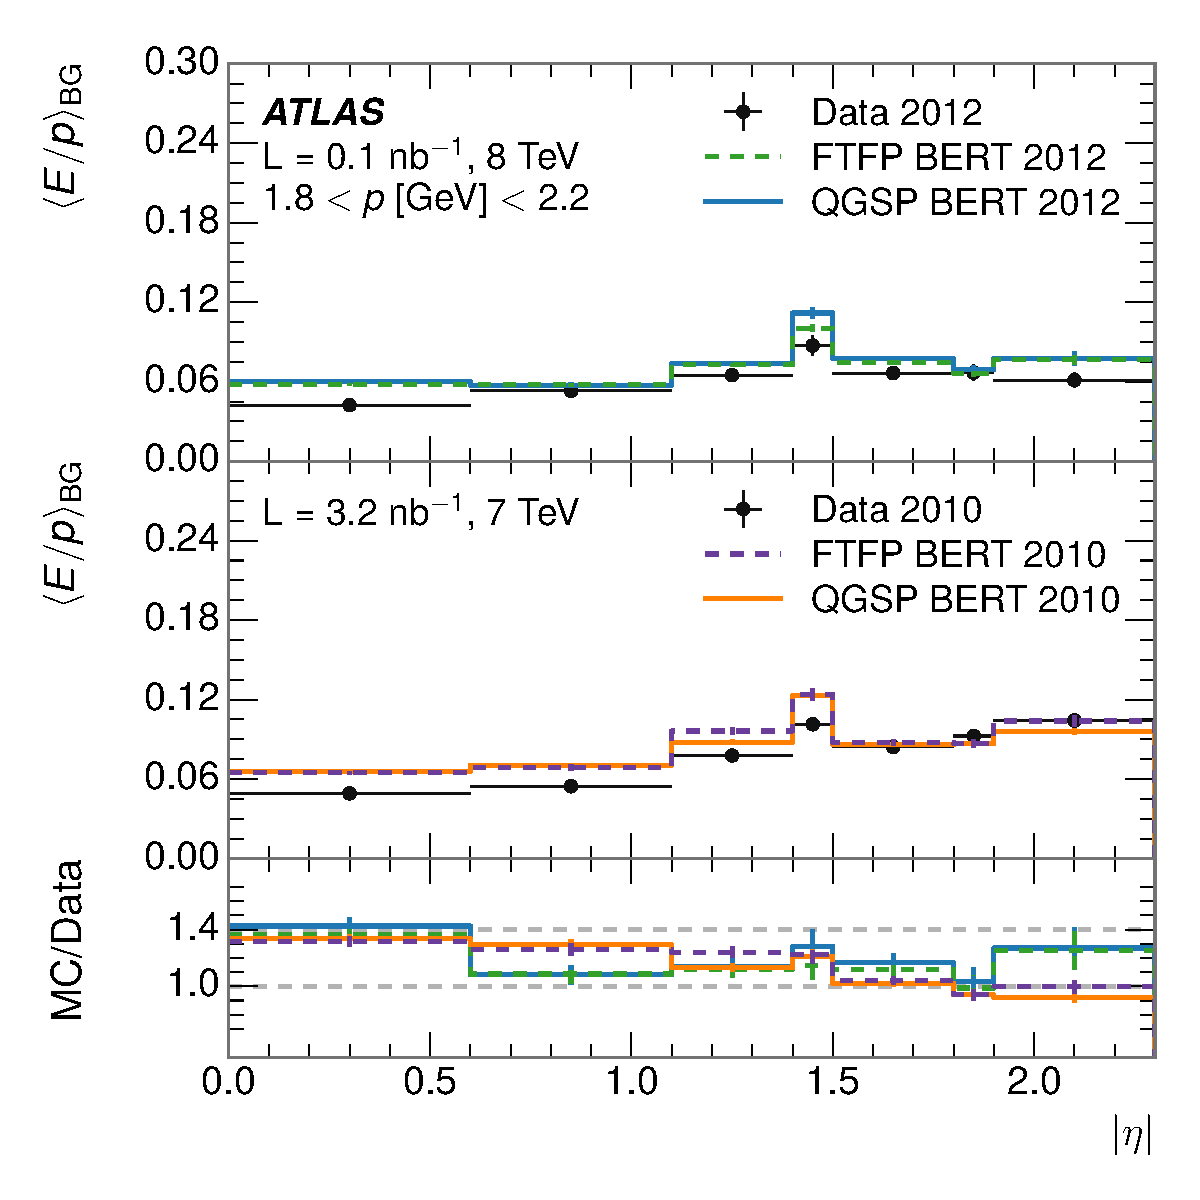
\includegraphics[width=\halffig]{figures/dvmc_epbg_layer01_calib01_p04_q00_nc00_trt02.pdf}
}
\caption{\epbg as a function of the track momentum for tracks with (a) $|\eta| < 0.6$, (b) $0.6 < |\eta| < 1.1$, and as a function of the track pseudorapidity for tracks with (c) $1.2 < p / \GeV < 1.8$, (d) $1.8 < p / \GeV < 2.2$.}
\label{fig:eoverp_background}
\end{figure}

\subsection{Corrected Response}
\label{sec:response}

Figure~\ref{fig:eoverp_corrected} shows \epcor as a function of momentum for several bins of pseudorapidity. 
This corrected $\epcor \equiv \epav - \epbg$ measures the average calorimeter response without the contamination of neutral particles. 
It is the most direct measurement of calorimeter response in that it is the energy measured for fully isolated hadrons. 
The correction is performed separately in data and simulation, so that the mismodeling of the neutral background in simulation is removed from the comparison of response. 
The simulation overestimates the response at low momentum by about 5\%, an effect that can be mostly attributed to the underestimation of the zero fraction mentioned previously.
For $|\eta| < 0.6$, the data-simulation agreement has a larger discrepancy by about 5\% for 2010 than 2012, although this is not reproduced in at higher pseudorapidity. 

\begin{figure}[htbp]
\centering
\subfloat[]{
  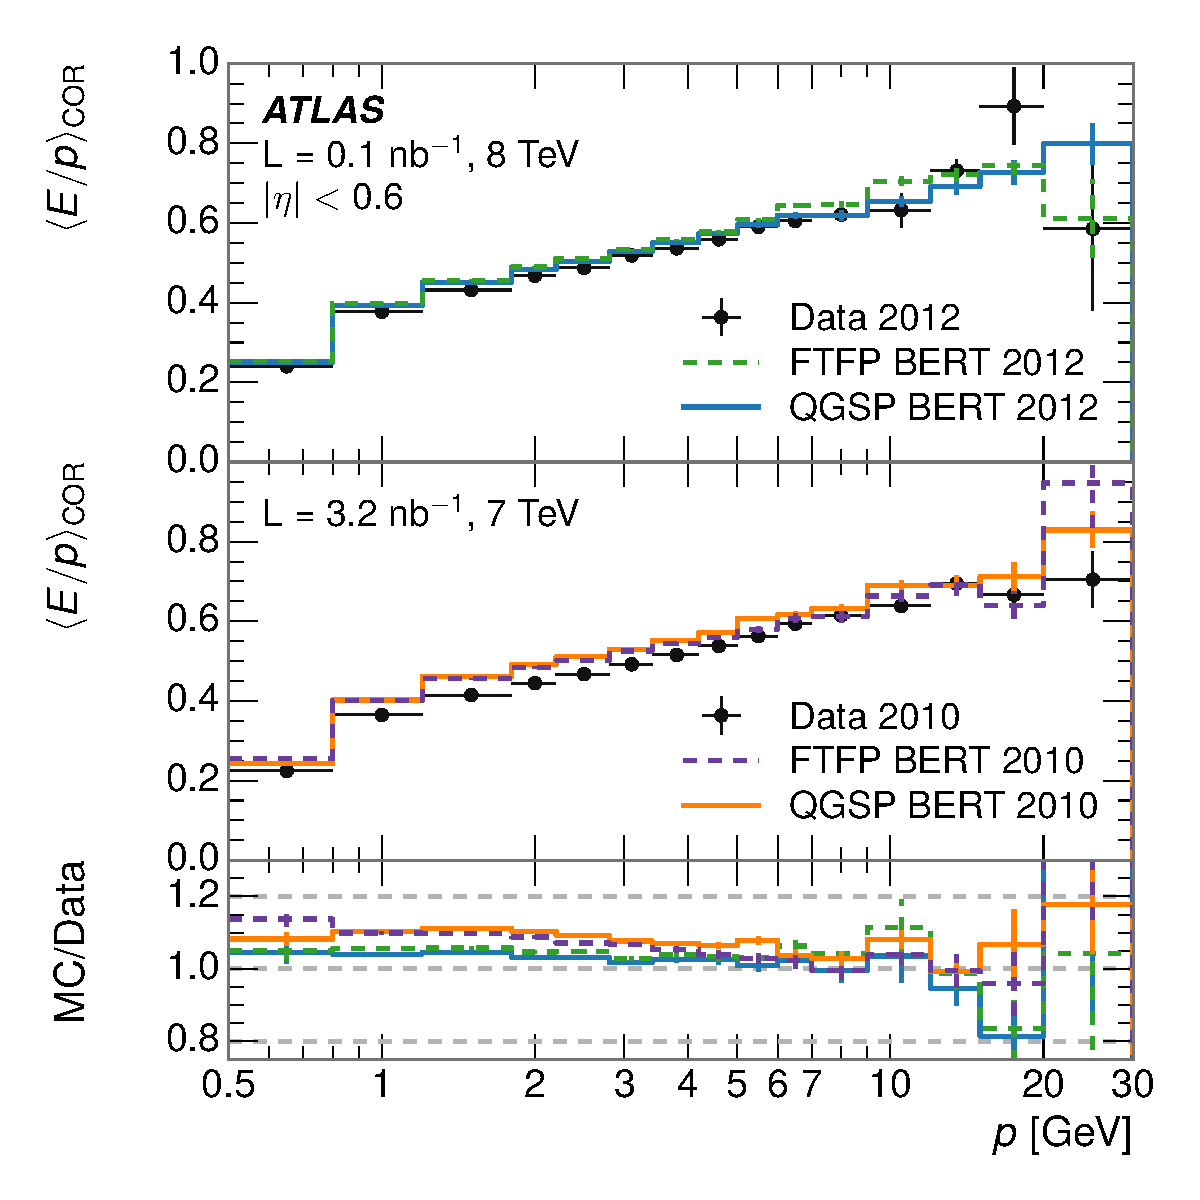
\includegraphics[width=\halffig]{figures/dvmc_epcor_layer01_calib01_eta01_q00_nc00_trt02.pdf}
}
~
\subfloat[]{
  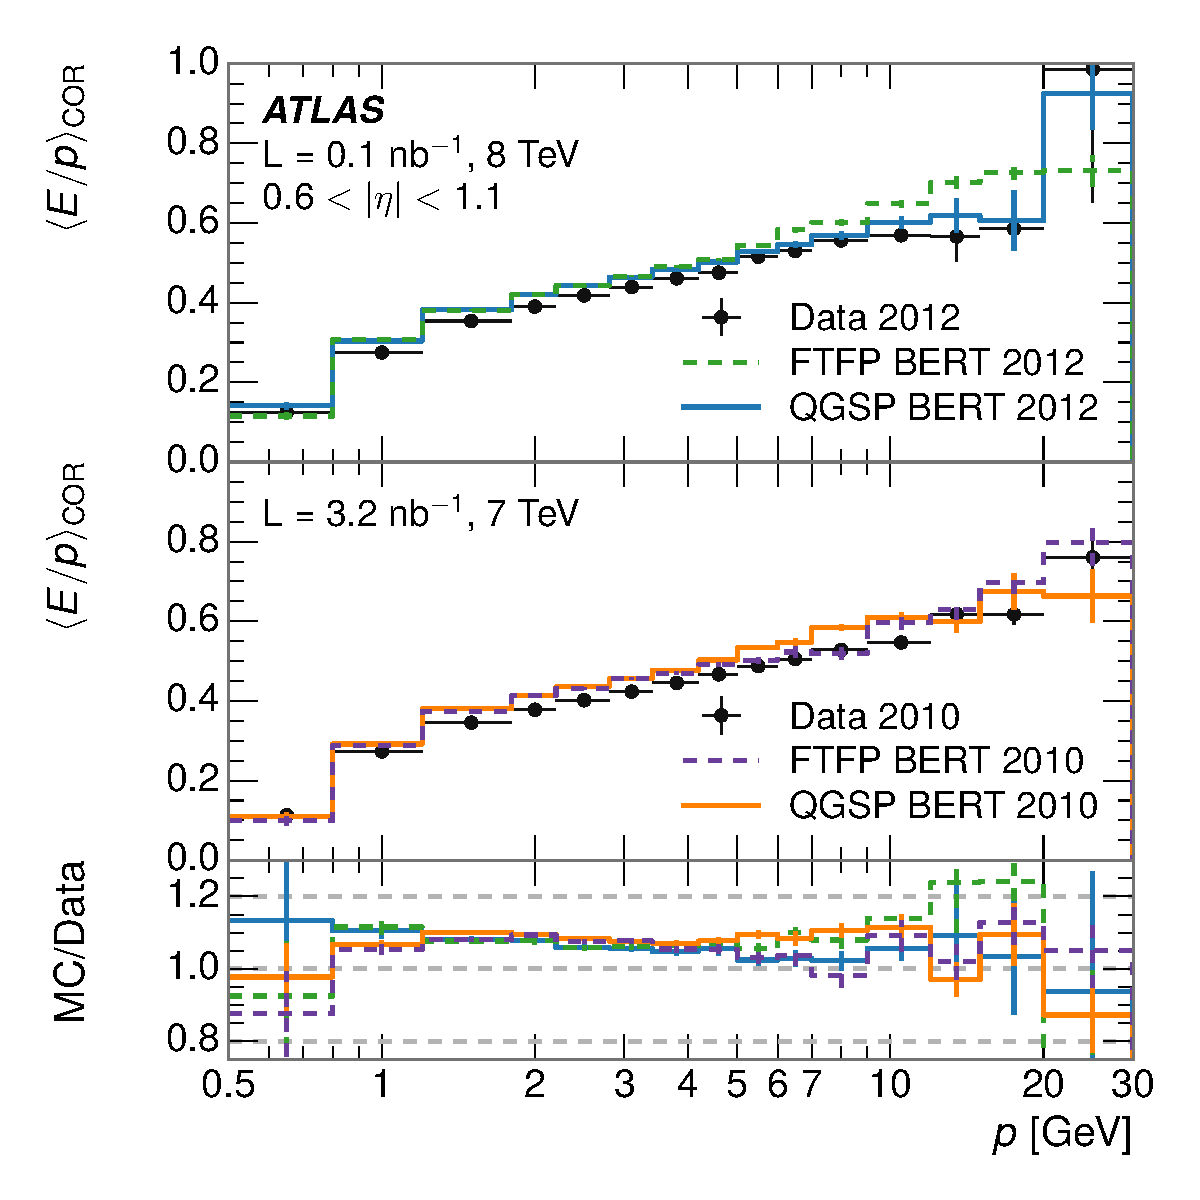
\includegraphics[width=\halffig]{figures/dvmc_epcor_layer01_calib01_eta02_q00_nc00_trt02.pdf}
}
\\
\subfloat[]{
  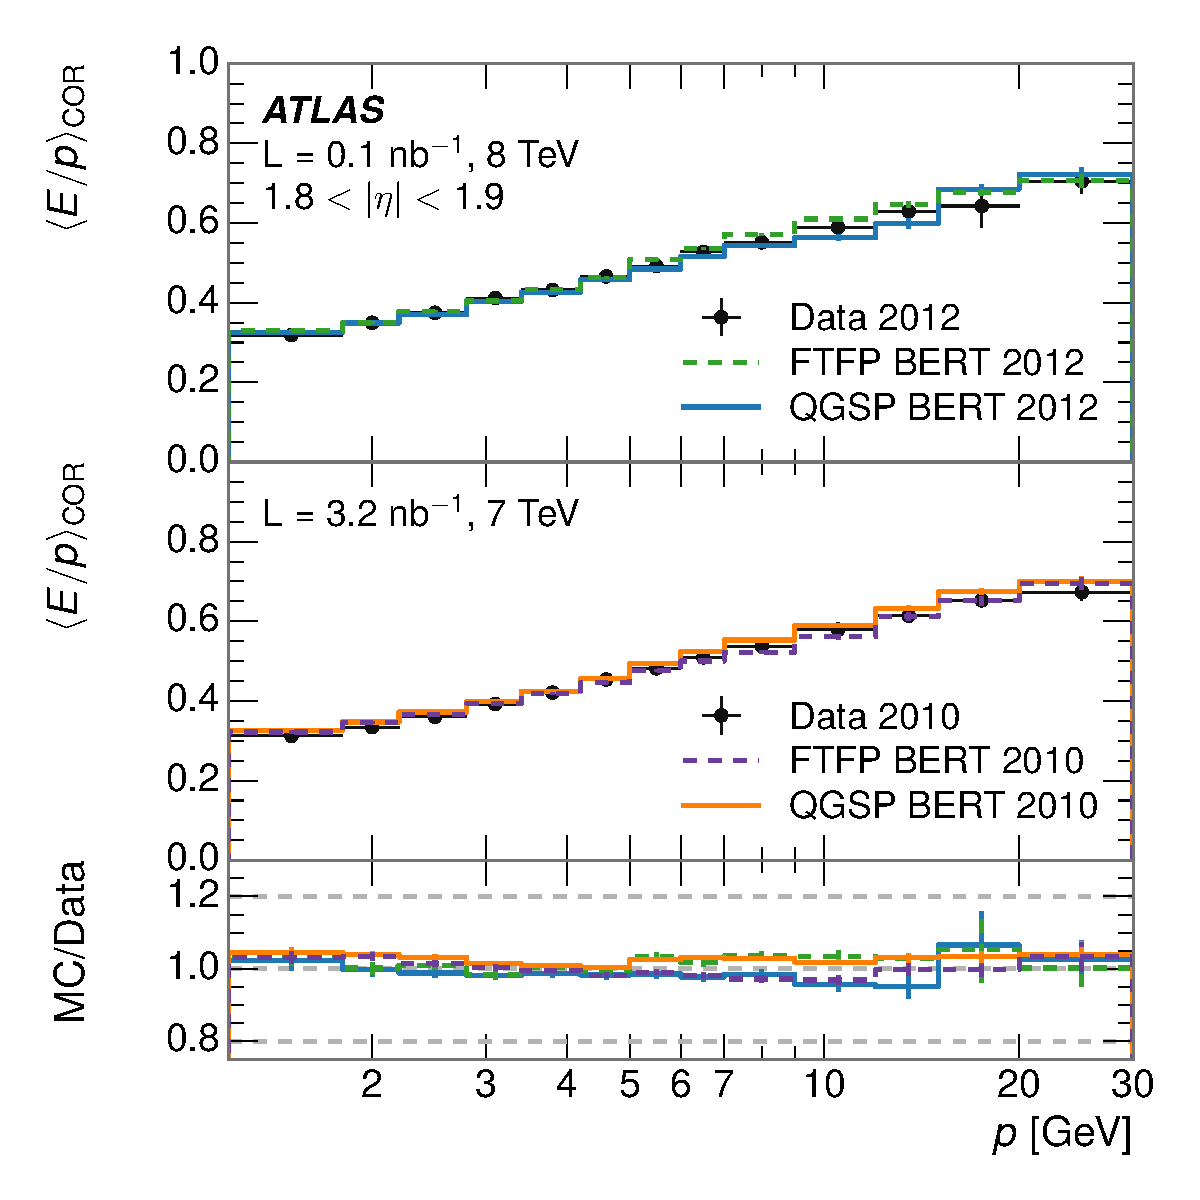
\includegraphics[width=\halffig]{figures/dvmc_epcor_layer01_calib01_eta06_q00_nc00_trt02.pdf}
}
~
\subfloat[]{
  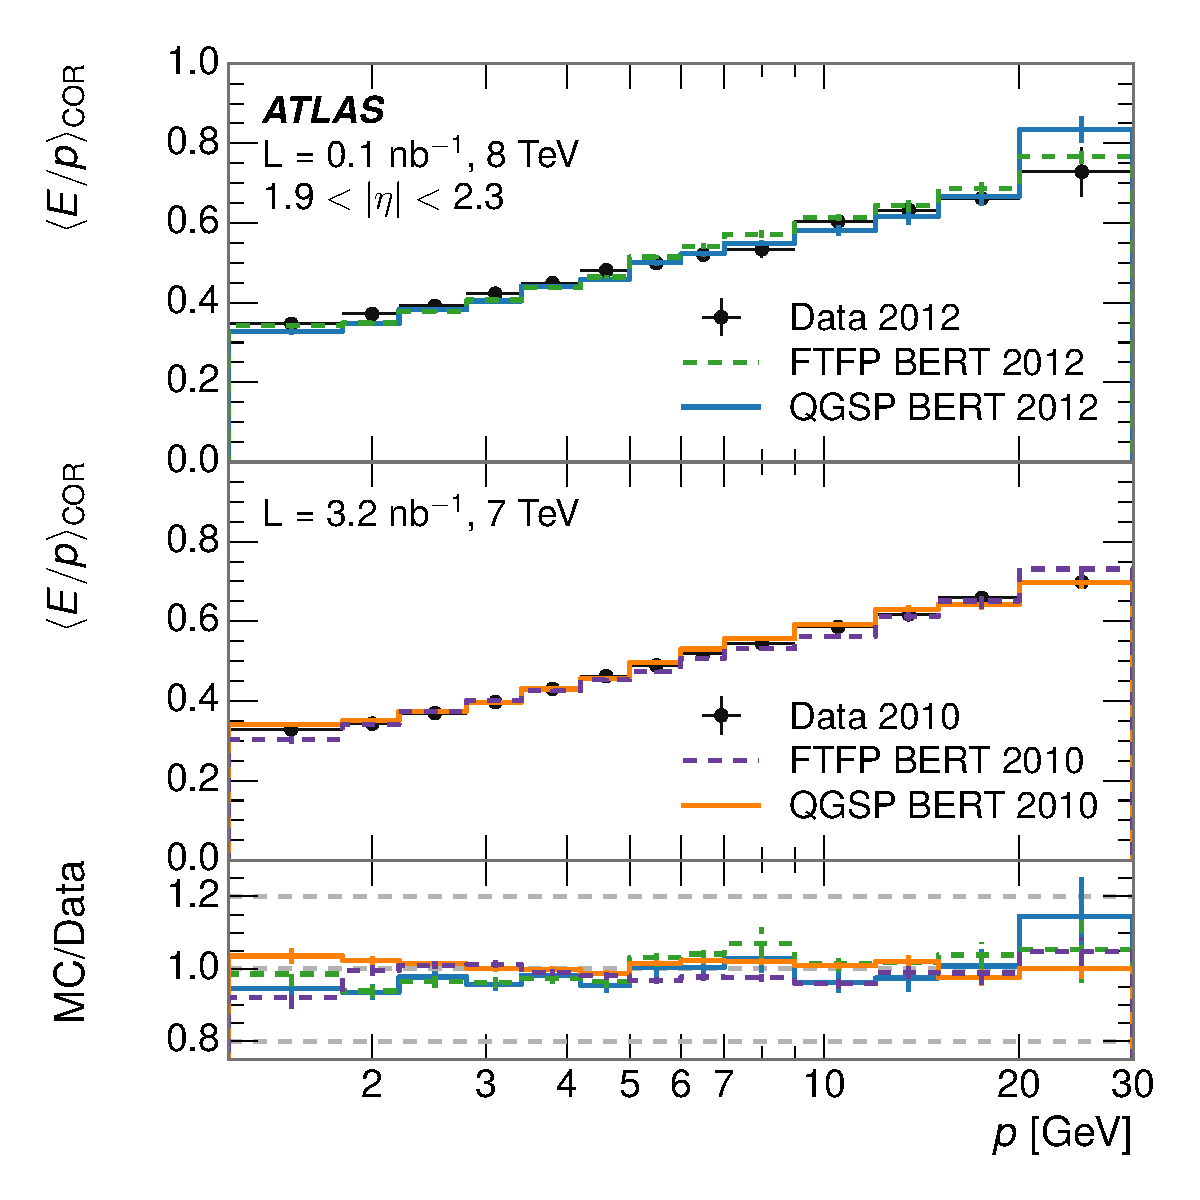
\includegraphics[width=\halffig]{figures/dvmc_epcor_layer01_calib01_eta07_q00_nc00_trt02.pdf}
}
\caption{\epcor as a function of track momentum, for tracks with (a) $|\eta| < 0.6$, (b) $0.6 <  |\eta| < 1.1$, (c) $1.8 <  |\eta| < 1.9$, and (d) $1.9 <  |\eta| < 2.3$. }
\label{fig:eoverp_corrected}
\end{figure}


The response measurement above used topological clustering at the EM scale, that is clusters were formed to measure energy but no corrections were applied to correct for expected effects like energy lost outside of the cluster or in uninstrumented material. 
It is also interesting to measure \epcor using \ac{LCW} energies, which accounts for those effects by calibrating the energy based on the properties of the cluster such as energy density and depth in the calorimeter.
Figure~\ref{fig:eoverp_corrected_lcw} shows these distributions for tracks with zero or more clusters and separately for tracks with one or more clusters.
The calibration moves the mean value of \epcor significantly closer to 1.0 as desired, but the discrepancy between data and simulation remains in the comparison that includes tracks with zero associated clusters.
The agreement between data and simulation improves noticeably when at least one cluster is required, as this removes the contribution from the mismodeling of the zero fraction. 

\begin{figure}[h]
\centering
\subfloat[]{
  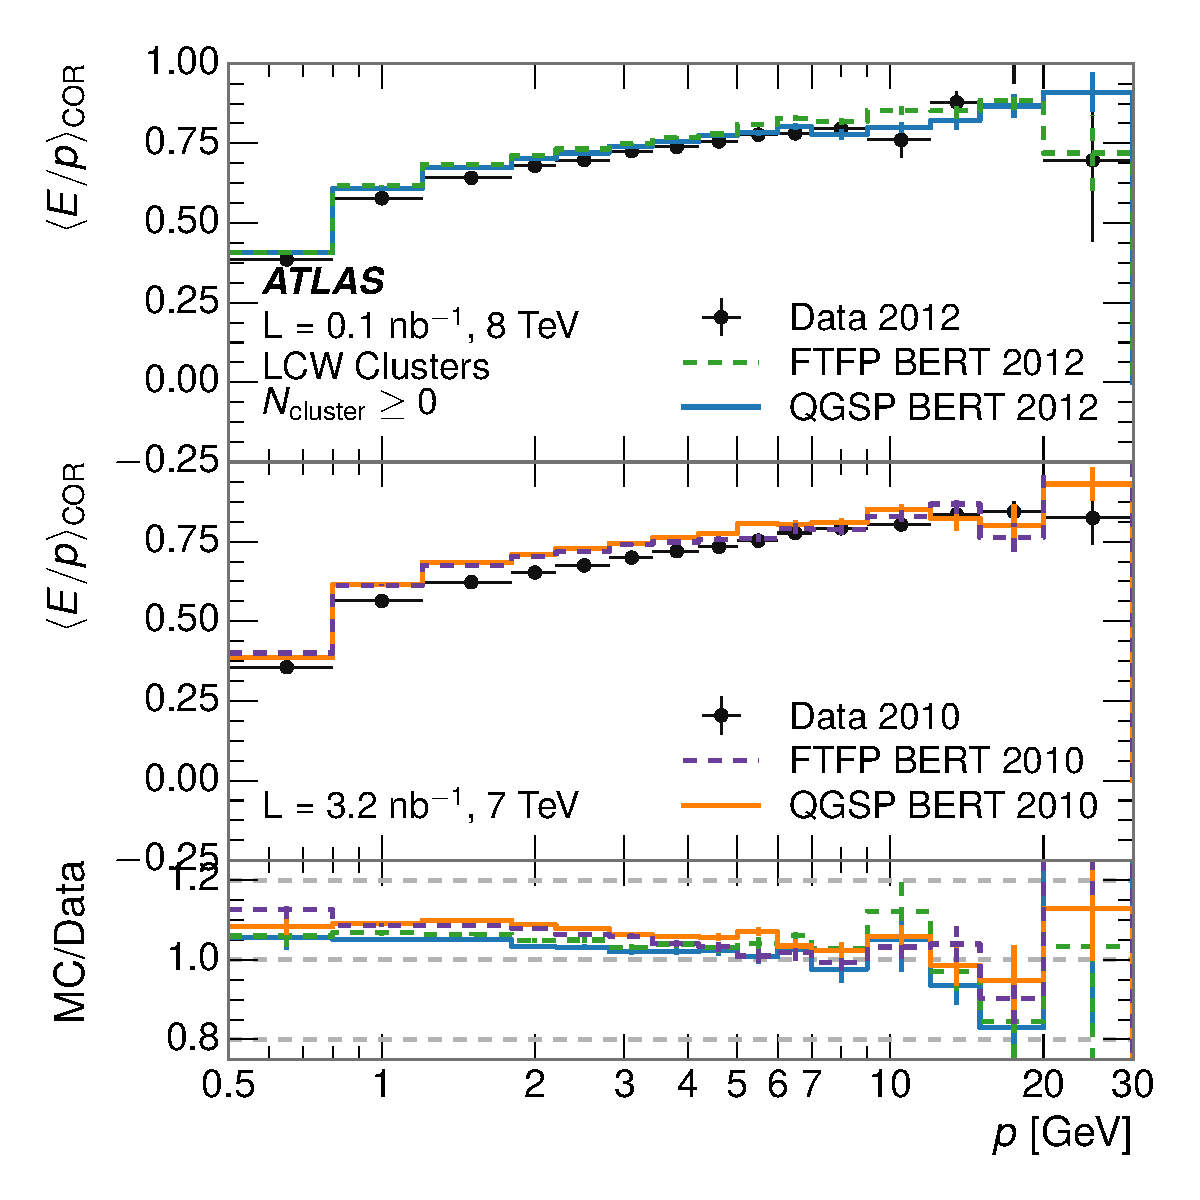
\includegraphics[width=\halffig]{figures/dvmc_epcor_layer01_calib02_eta01_q00_nc00_trt02.pdf}
}
~
\subfloat[]{
  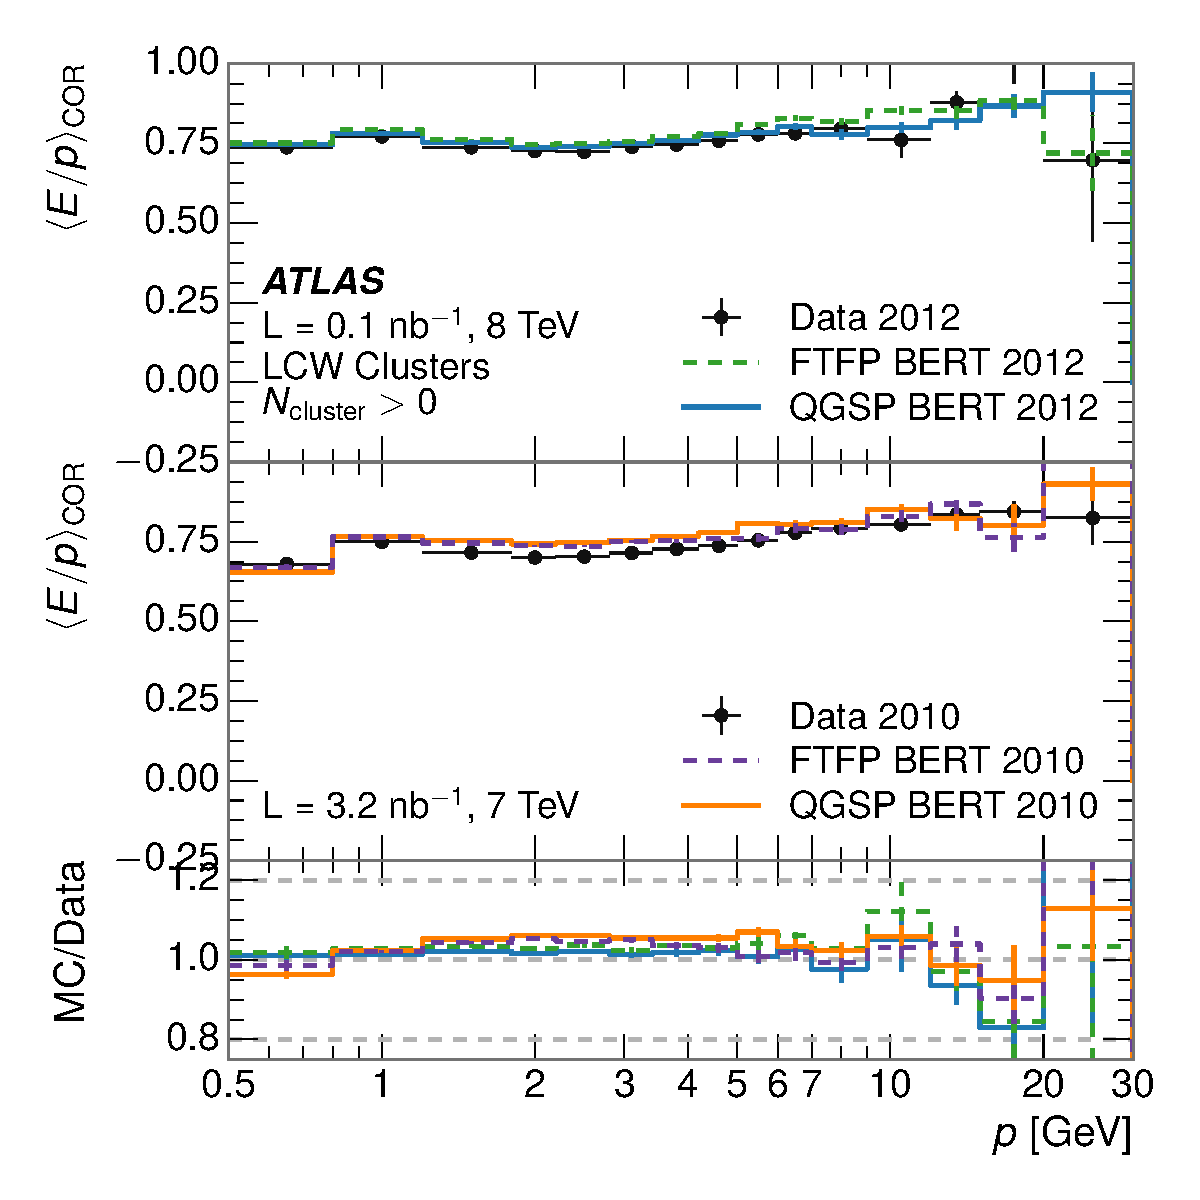
\includegraphics[width=\halffig]{figures/dvmc_epcor_layer01_calib02_eta01_q00_nc02_trt02.pdf}
}
\caption{\epcor calculated using LCW-calibrated topological clusters as a function of track momentum for tracks with (a) zero or more associated topological clusters or (b) one or more associated topological clusters.}
\label{fig:eoverp_corrected_lcw}
\end{figure}


\subsection{Additional Studies}
\label{sec:additional}

As has been seen in several measurements in previous sections, the simulation does not correctly model the chance of a low momentum hadron to reach the calorimeter.
Because of the consistent discrepancy across pseudorapidity and interaction lengths, this can be best explained by incomplete understanding of hadronic interactions with the detector~\cite{PERF-2015-05}.
For example, a hadron that scatters off of a nucleus in the inner detector can be deflected through a significant angle and not reach the expected location in the calorimeter.
In addition, these interactions can produce secondary particles that are difficult to model.

The requirement used throughout the previous sections  on the number of hits in the TRT reduces these effects by preferentially selecting tracks that do not undergo nuclear interactions.
It is interesting to check how well the simulation models tracks with low numbers of TRT hits, which selects tracks that are more likely to have undergone a hadronic interaction.
Figure~\ref{fig:eoverp_trt} compares the distributions with $N_{\mathrm{TRT}} < 20$ to $N_{\mathrm{TRT}} > 20$ for real and simulated particles\footnote{The distribution with $N_{\mathrm{TRT}} > 20$ is the same as shown in Figure~\ref{fig:eoverp_corrected} (a) and is included again here for the comparison.}.
As expected, the tracks with fewer hits are poorly modeled in the simulation as \epcor differs by as much as 25\% at low momentum.
They also have significantly lower \epcor on average, because they are much less likely to have an associated cluster.

\begin{figure}[h]
\centering
\subfloat[]{
  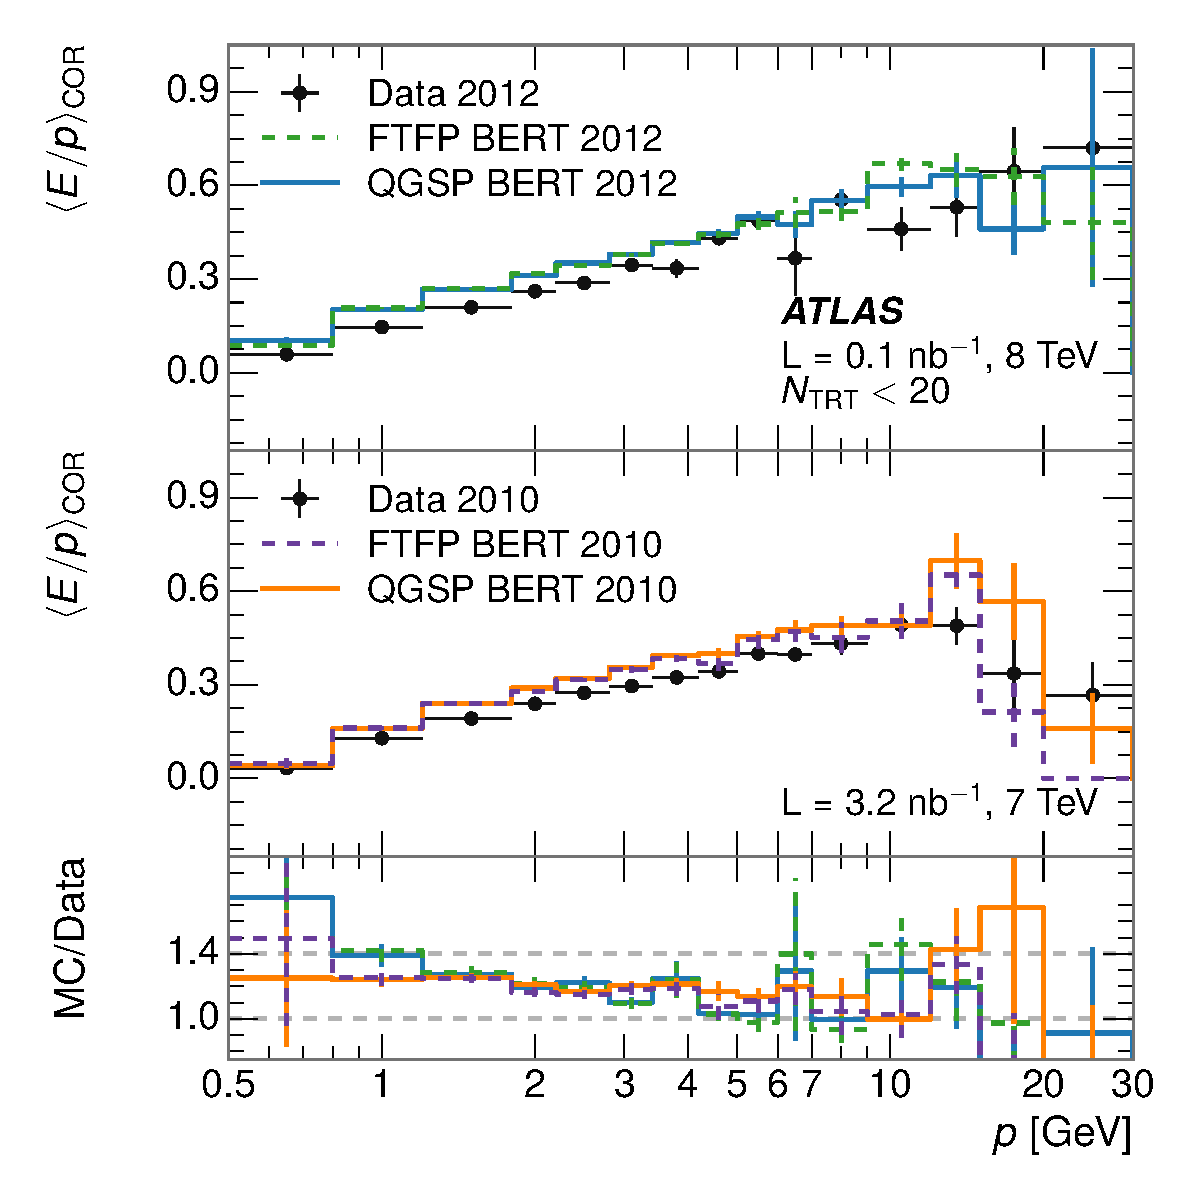
\includegraphics[width=\halffig]{figures/trt_dvmc_epcor_layer01_calib01_eta01_q00_nc00_trt01.pdf}
}
~
\subfloat[]{
  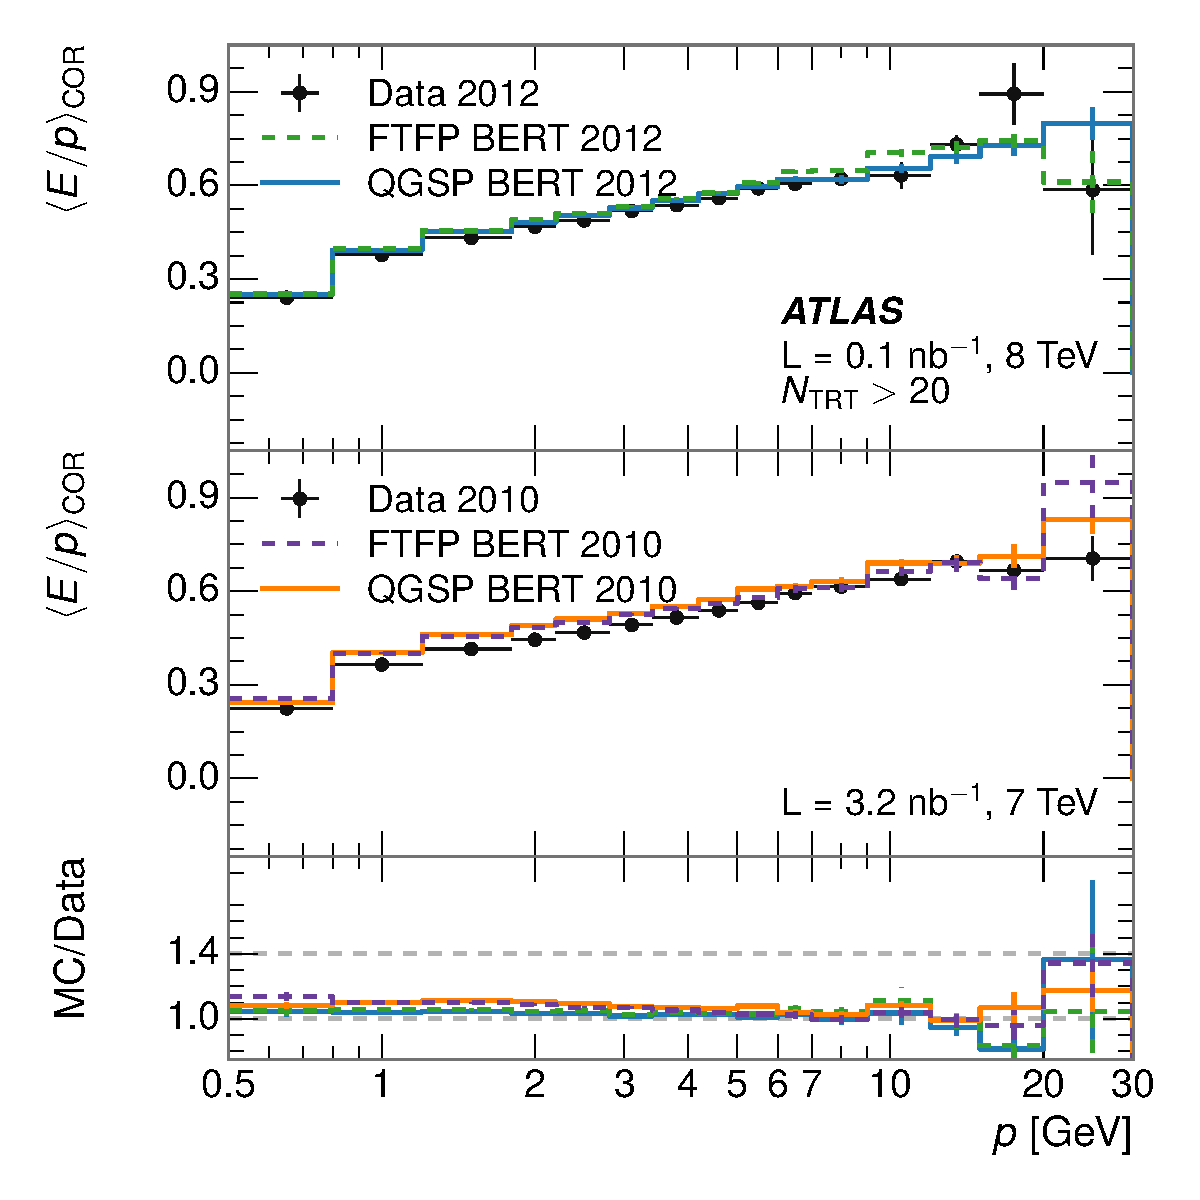
\includegraphics[width=\halffig]{figures/trt_dvmc_epcor_layer01_calib01_eta01_q00_nc00_trt02.pdf}
}
\caption{Comparison of the \epcor for tracks with (a) less than and (b) greater than 20 hits in the TRT.}
\label{fig:eoverp_trt}
\end{figure}

Another interesting aspect of the simulation is the description of antiprotons at low momentum, where \QGSP and \FTFP have significant differences.
This can be seen to have an effect in the inclusive response measurement when separated into positive and negative charge.
The \epcor distributions for positive and negative particles are shown in Figure~\ref{fig:eoverp_corrected_charge}, where a small difference between \QGSP and \FTFP can be seen in the distribution for negative tracks.
The figure also includes data, and the simulation overestimates \epcor mostly due to an underestimation in zero fraction.
There is an approximately 5\% difference between the 2010 and 2012 simulated events.
The difference between positive and negative particles is demonstrated more clearly in Figure~\ref{fig:eoverp_charge}, which shows the \ep distribution in the two simulations separated by charge.
There is a small difference around $\ep > 1.0$, which can be explained by the additional energy deposited by the annihilation of the antiproton in the calorimeter that is modeled well only in \FTFP.
This is also explored with data using identified antiprotons in Section~\ref{sec:identified}. 

\begin{figure}[h]
\centering
\subfloat[]{
  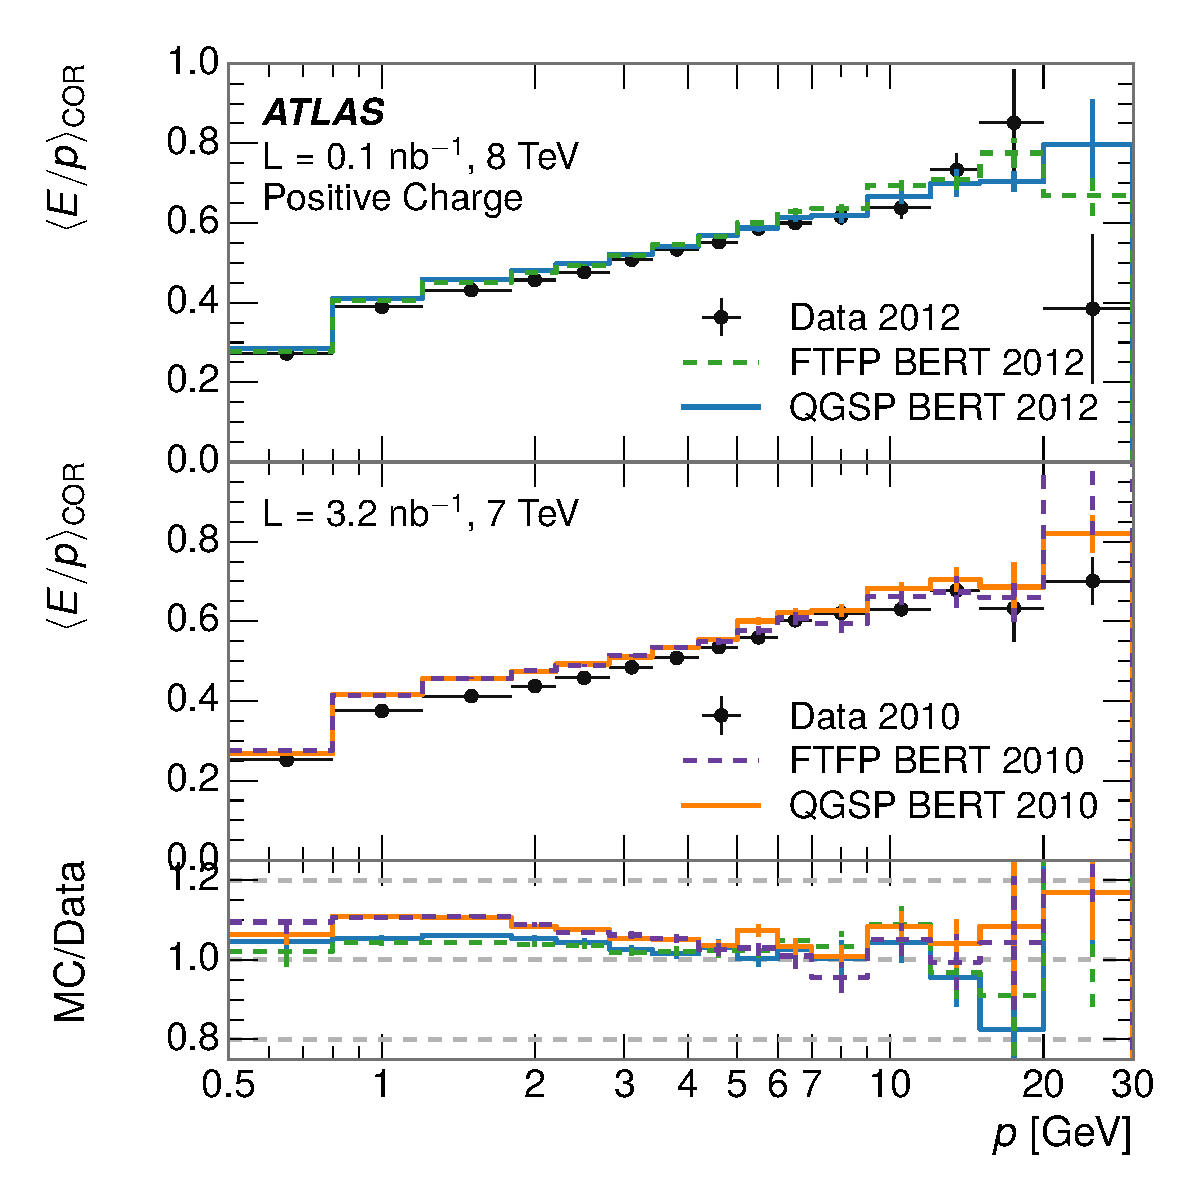
\includegraphics[width=\halffig]{figures/dvmc_epcor_layer01_calib01_eta01_q02_nc00_trt02.pdf}
}
~
\subfloat[]{
  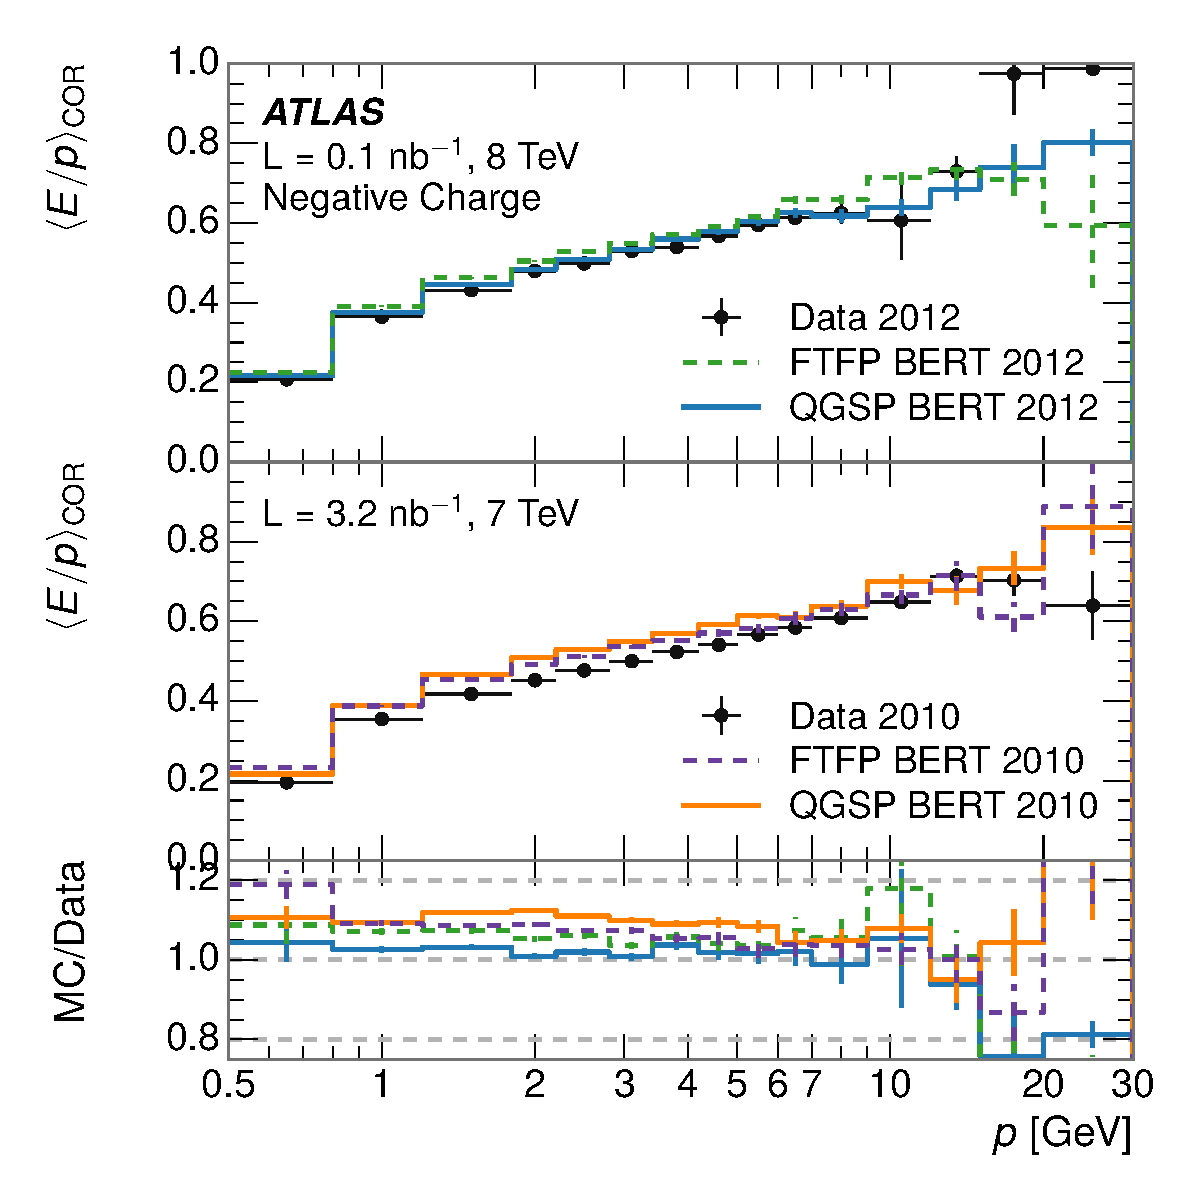
\includegraphics[width=\halffig]{figures/dvmc_epcor_layer01_calib01_eta01_q01_nc00_trt02.pdf}
}
\caption{Comparison of the \epcor for (a) positive and (b) negative tracks as a function of track momentum for tracks with $|\eta|<0.6$.}
\label{fig:eoverp_corrected_charge}
\end{figure}

\begin{figure}[ht]
\centering
\subfloat[]{
  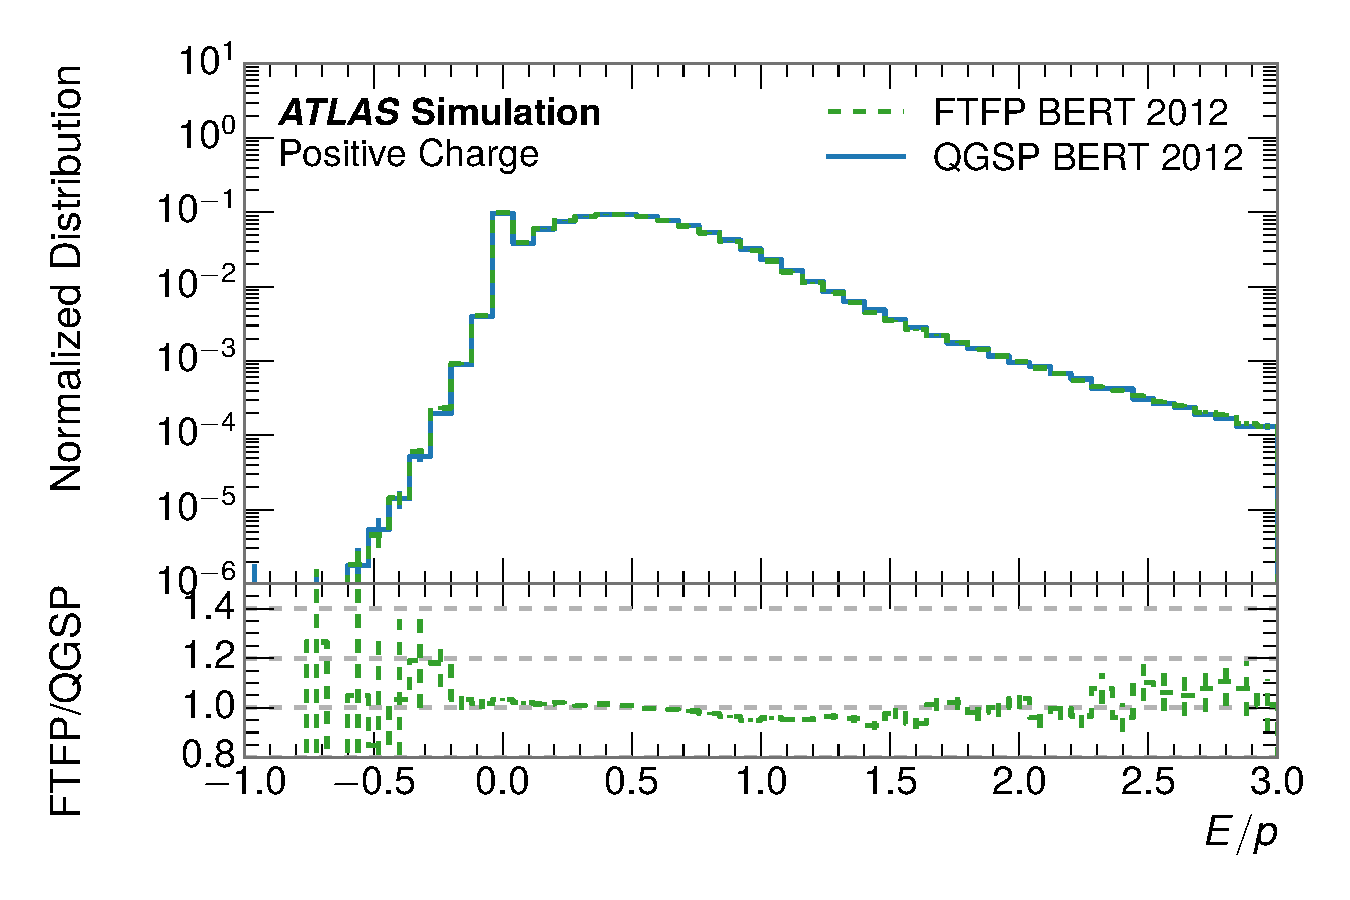
\includegraphics[width=\halffig]{figures/eoverp_TOT_eta01_p03_q02_MC.pdf}
}
~
\subfloat[]{
  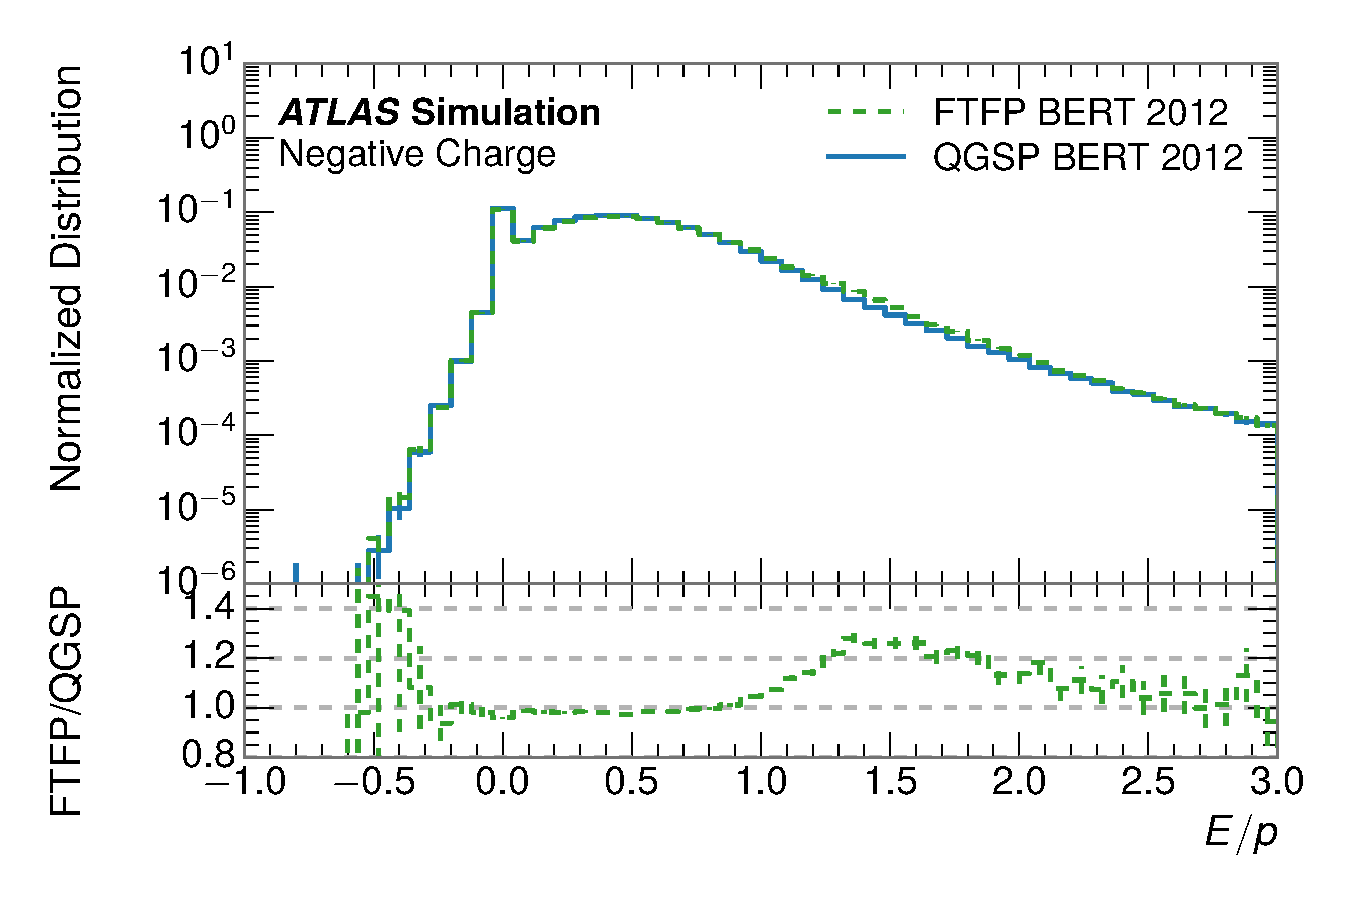
\includegraphics[width=\halffig]{figures/eoverp_TOT_eta01_p03_q01_MC.pdf}
}
\caption{ Comparison of the \ep distributions for (a) positive and (b) negative tracks with $0.8< p/\GeV<1.2$ and $|\eta|<0.6$, in simulation with the \texttt{FTFP\_BERT} and \texttt{QGSP\_BERT} physics lists.}
\label{fig:eoverp_charge}
\end{figure}

The \epav results in previous sections have considered the electromagnetic and hadronic calorimeters together as a single energy measurement, to emphasize the total energy deposited for a given particle. 
However, the deposits in each calorimeter are measured separately and \epav can be constructed for each layer separately. 
As the layers are composed of different materials and are modeled separately in the detector geometry, confirmation that the simulation matches the data well in each layer adds confidence in both the description of hadronic interactions with the two different materials and also the geometric description of each. 

The technique discussed in Section~\ref{sec:neutral_bg} for selecting \ac{MIP}s in the electromagnetic calorimeter is also useful in studying deposits in the hadronic calorimeter.
The tracks selected with the \ac{MIP} requirements deposit almost all of their energy exclusively in the hadronic calorimeter.
Figure~\ref{fig:epav_hcal} shows \epav$_\mathrm{RAW}^\mathrm{Had}$, where RAW indicates that no correction has been applied for neutral backgrounds and Had indicates that only clusters for the hadronic calorimeter are included\footnote{The RAW and COR versions of \epav in this case are the same, as the neutral background is negligible in that calorimeter layer.}.
The distributions are shown both for the original EM scale calibration and after LCW calibration.
The data and simulation agree very well in this comparison, except in the lowest momentum bin where there is a 5\% discrepancy that has already been seen in the measurements in Section~\ref{sec:response}.

\begin{figure}[h]
\centering
\subfloat[]{
  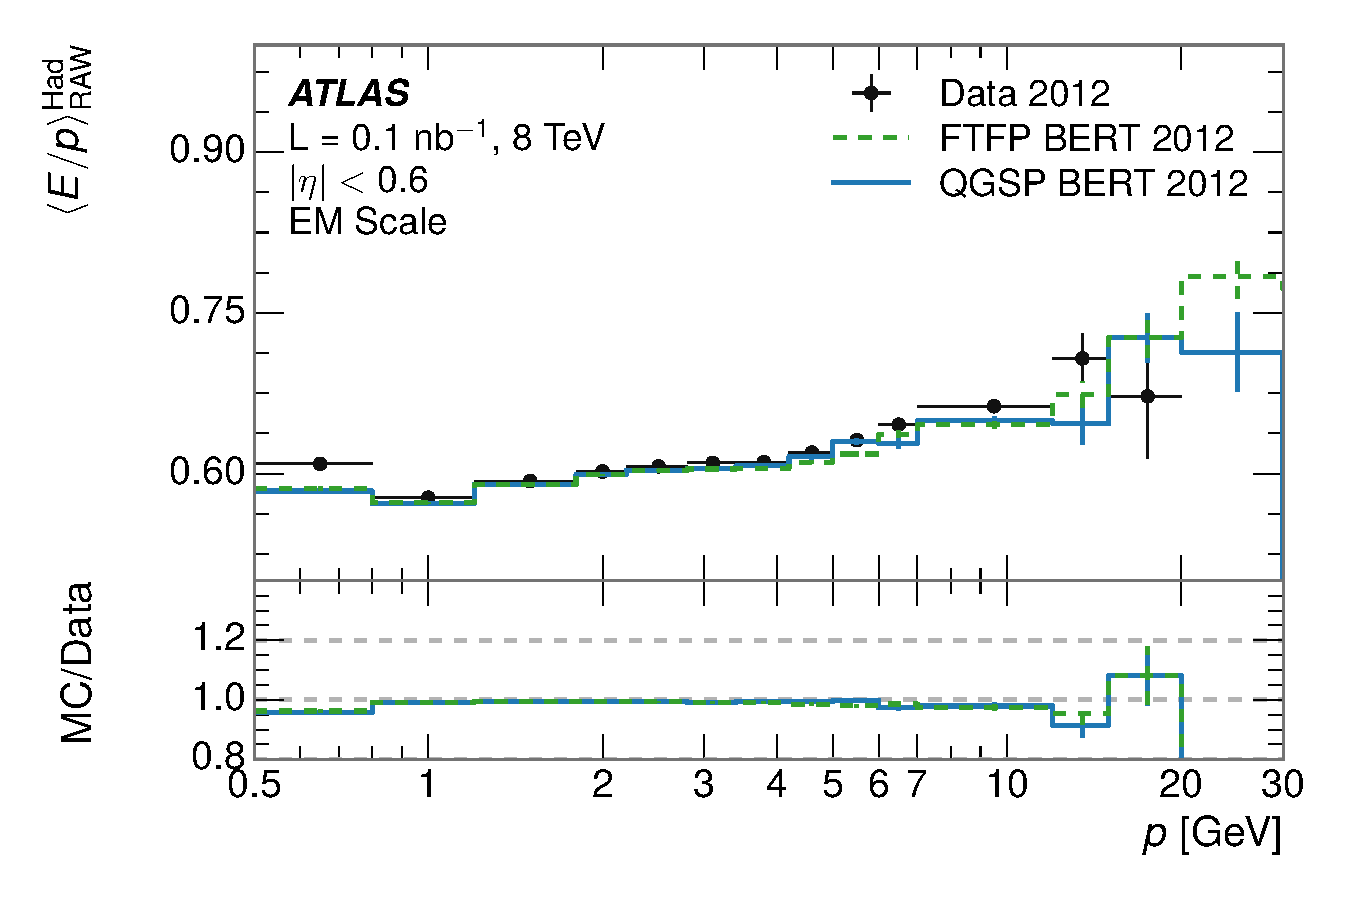
\includegraphics[width=\halffig]{figures/EPvsP_raw_HCal_EMscale_eta_06.pdf}
}
~
\subfloat[]{
  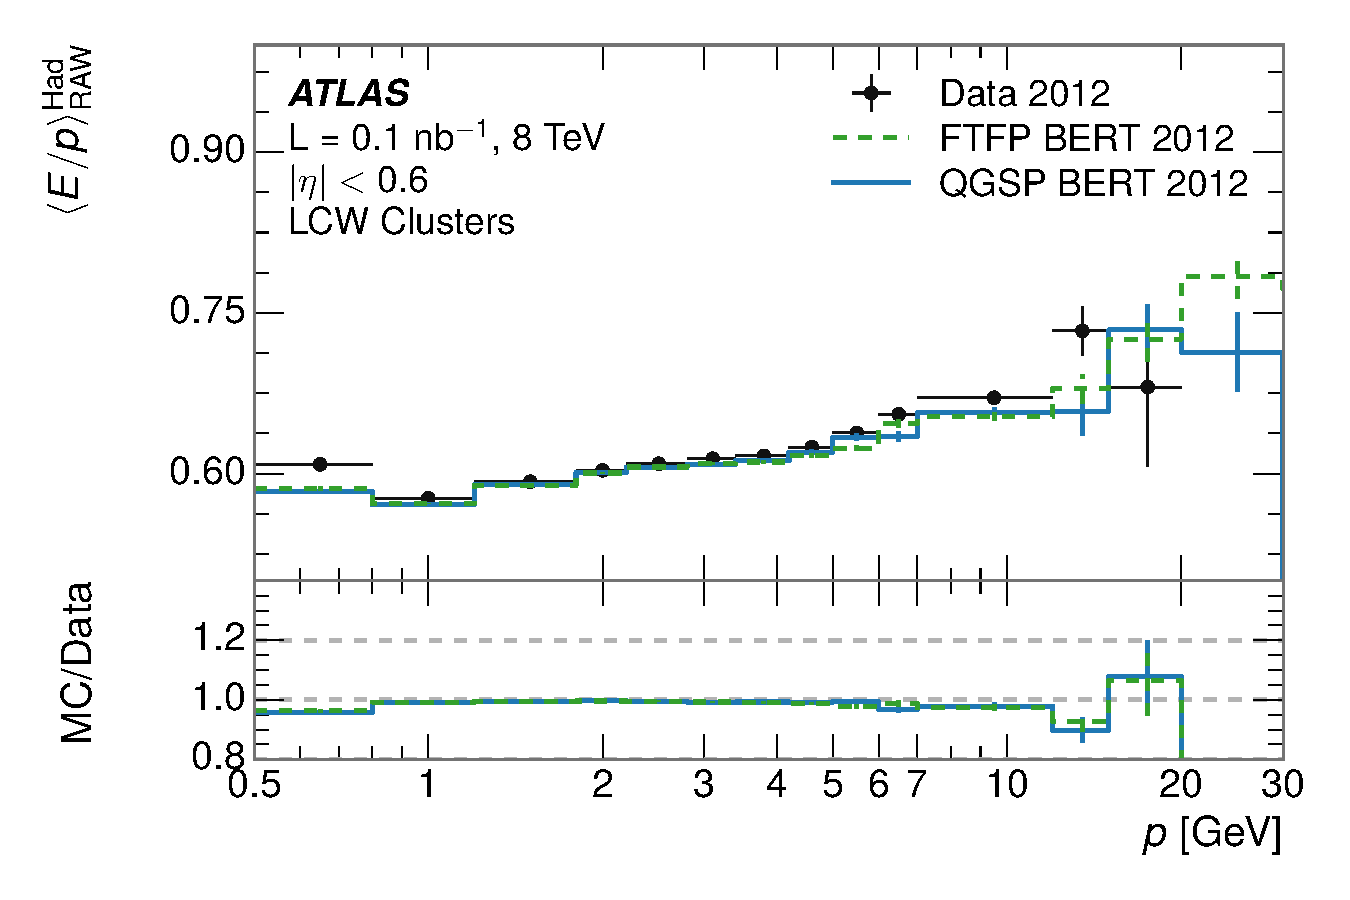
\includegraphics[width=\halffig]{figures/EPvsP_raw_HCal_LCW_eta_06.pdf}
}
\caption{Comparison of the response of the hadronic calorimeter as a function of track momentum (a) at the EM-scale and (b) after the LCW calibration.}
\label{fig:epav_hcal}
\end{figure}

A similar comparison can be made in the electromagnetic calorimeter by selecting particles which have no associated energy in the hadronic calorimeter. 
These results are measured in terms of \epav$_{\mathrm{COR}}^{\mathrm{EM}}$, where EM designates that only clusters in the electromagnetic calorimeter are included and COR designates that the neutral background is subtracted as the neutral background is present in this case.
Figure~\ref{fig:epcor_ecal} shows the analogous comparisons to Figure~\ref{fig:epav_hcal} in the electromagnetic calorimeter.
The \epcor values are lower on average in the \ac{EM} calorimeter than in the hadronic calorimeter, which is an expected consequence of their different material types (discussed in Section~\ref{sec:calorimetry}). 
In this case the disagreement between data and simulation is more pronounced, with discrepancies as high as 5\% over a larger range of momenta.
This level of discrepancy indicates that the description of the electromagnetic calorimeter is actually the dominant source of discrepancy in the combined distributions in Section~\ref{sec:response}. 

\begin{figure}[htbp]
\centering
\subfloat[]{
  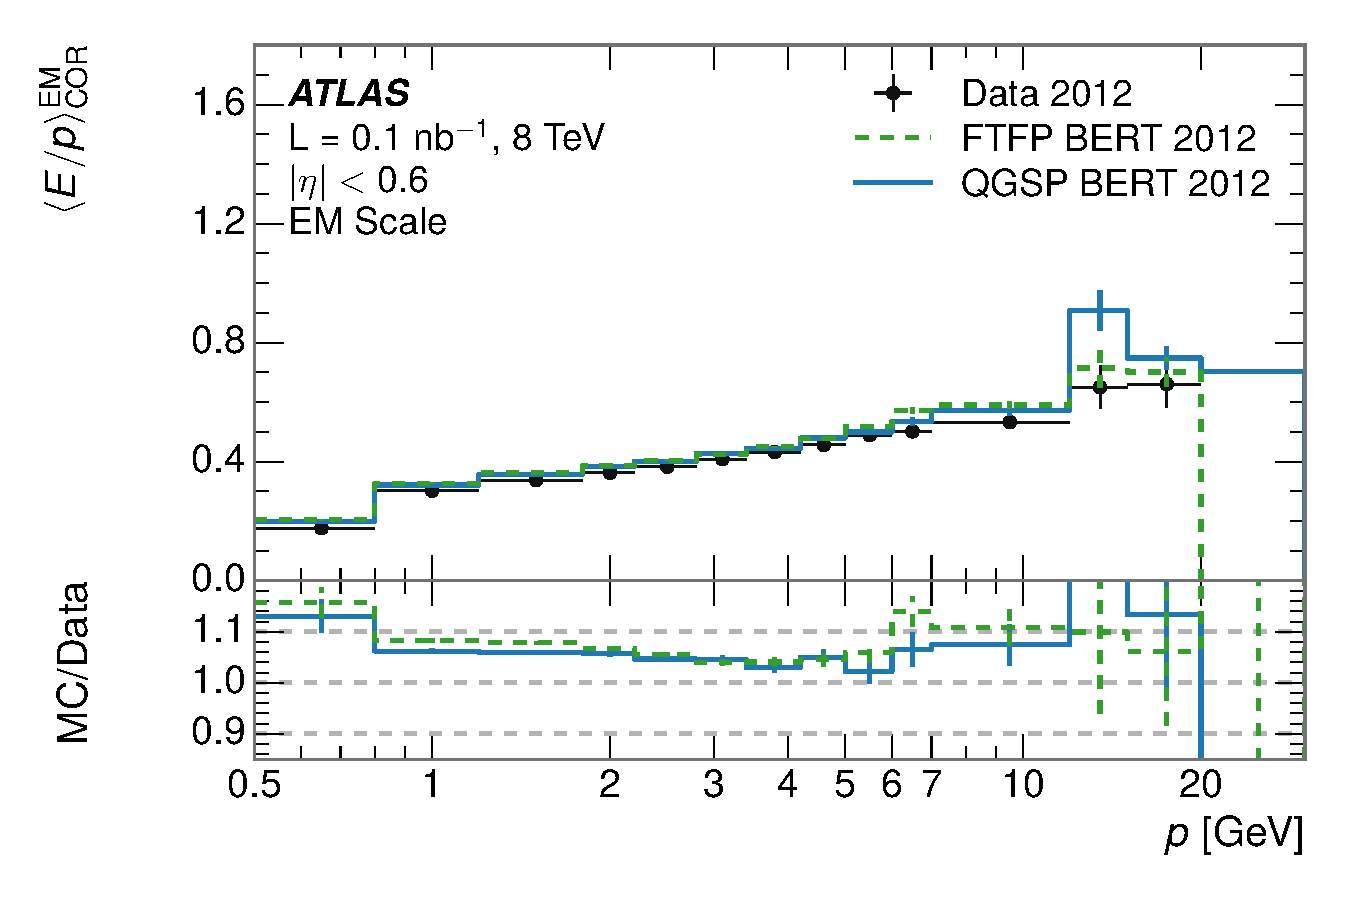
\includegraphics[width=\halffig]{figures/EPvsP_cor_ECal_EMscale_eta_06.pdf}
}
~
\subfloat[]{
  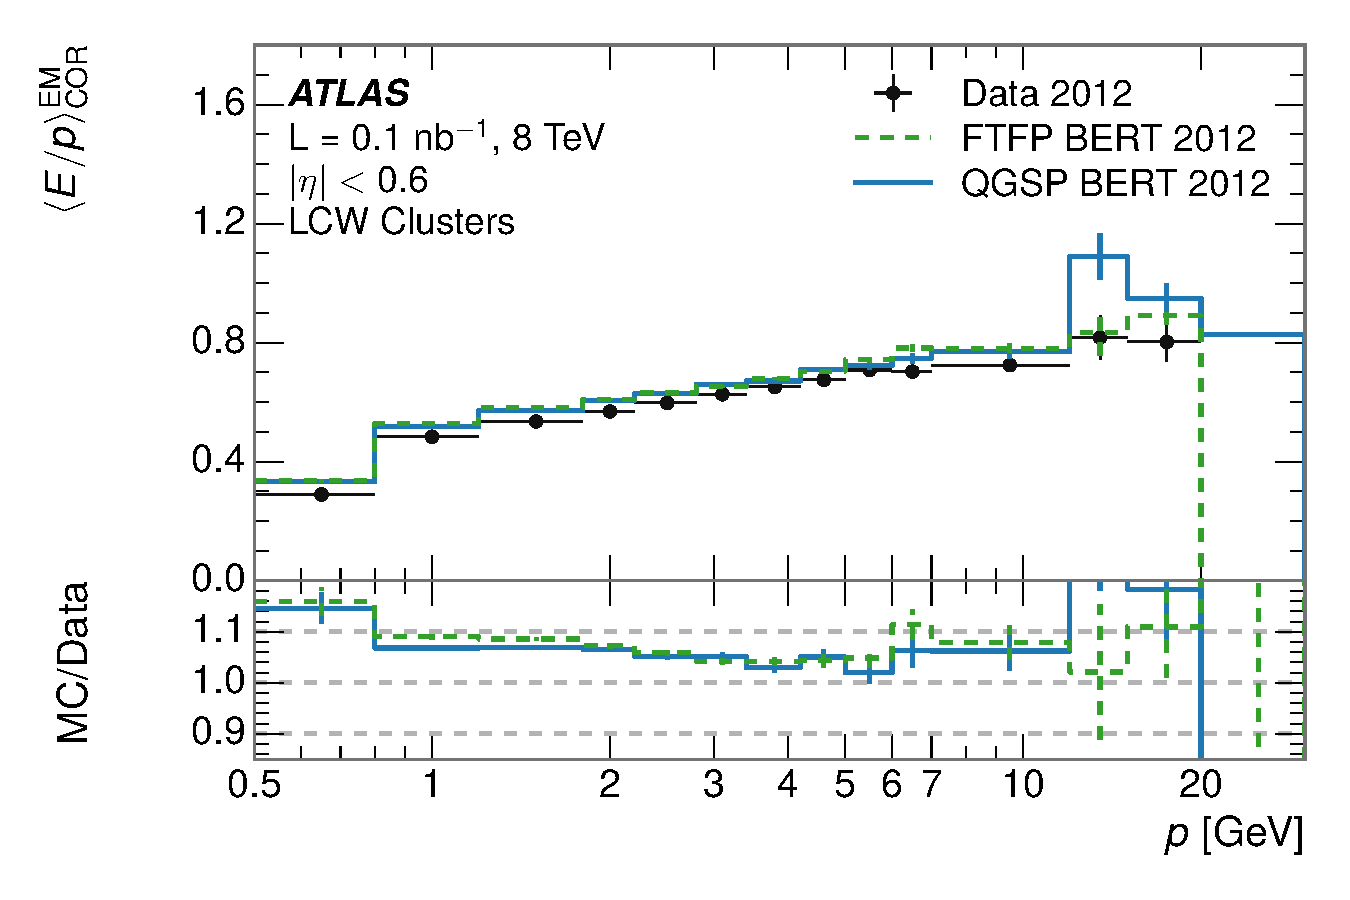
\includegraphics[width=\halffig]{figures/EPvsP_cor_ECal_LCW_eta_06.pdf}
}
\caption{Comparison of the response of the EM calorimeter as a function of track momentum (a) at the EM-scale and (b) with the LCW calibration.}
\label{fig:epcor_ecal}
\end{figure}

% ----------------------------------------

\section{Identified Particle Response}
\label{sec:identified}

The inclusive response measurement for hadrons can be augmented by measuring the response for specific particle species. 
The simulation models each particle type separately, and understanding the properties of each is important in constraining the uncertainty on jets. 
In order to select and measure specific hadrons, this section relies on the displaced decays of long-lived particles. 
Such decays can be identified by reconstructing secondary vertices with a requirement on mass.
In particular, \pL, \pLB, and \pKS can be used to select a pure sample of protons, antiprotons, and pions, respectively. 

\subsection{Decay Reconstruction}
The measurement of the response for identified particles uses the same selection as for inclusive particles (Section~\ref{sec:inclusive_selection}) with a few additions.
Each event used is required to have at least one secondary vertex, as described in Section~\ref{sec:vertices}, and the tracks are required to match to that vertex rather than the primary vertex.
Pions are selected from decays of $\pKS \rightarrow \pip \pim$, which is the dominant decay for \pKS to charged particles.
Protons are selected from decays of $\pL \rightarrow \pim \pP$ and antiprotons from $\pLB \rightarrow \pip \pAP$, which are similarly the dominant decays of \pL and \pLB to charged particles.
The species of parent hadron in these decays is determined by reconstructing the mass of the tracks associated to the secondary vertex.
The sign of the higher momentum decay particle can distinguish between \pL and \pLB, which of course have the same mass, as the proton or antiproton is kinematically favored to have higher momentum.
The proton or antiproton will carry the higher momentum above 95\% of the time.
Examples of the reconstructed masses used to select these decays are shown in Figure~\ref{fig:identified_mass}. 
The mass peaks in data and both simulation models are very similar.

\begin{figure}[htbp]
\centering
\subfloat[]{
  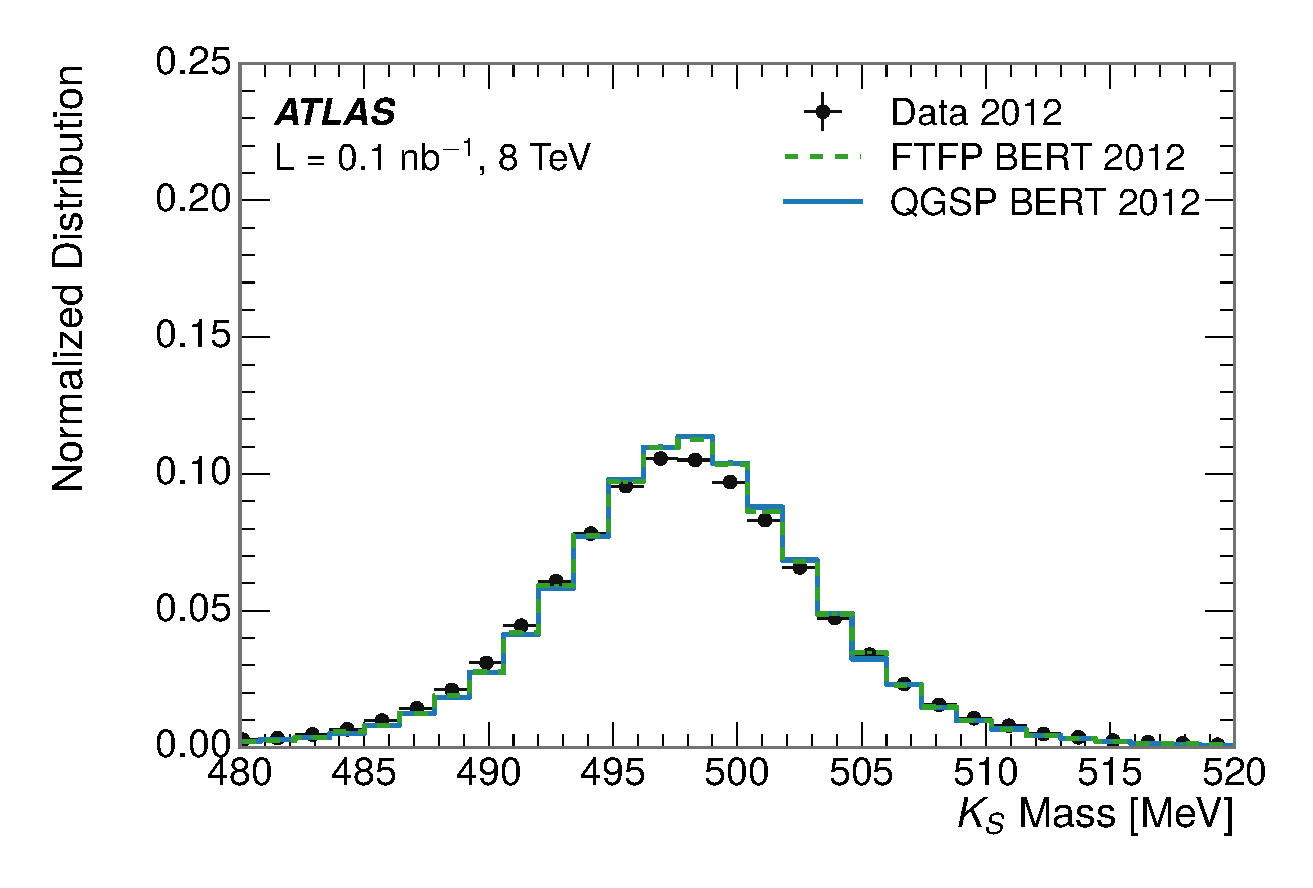
\includegraphics[width=\halffig]{figures/mass_kshort_eta01.pdf}
}
\\
\subfloat[]{
  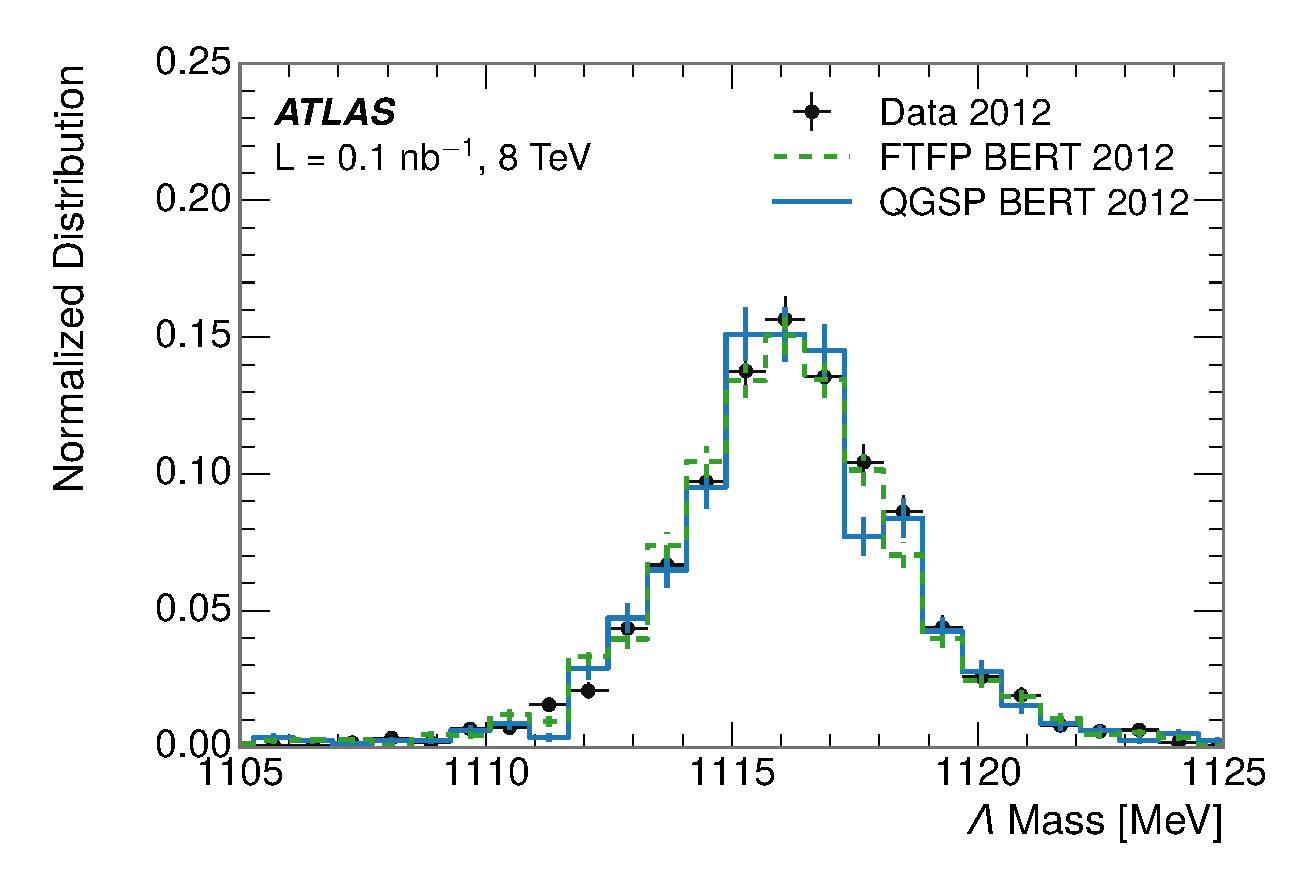
\includegraphics[width=\halffig]{figures/mass_lambda_eta01.pdf}
}
~
\subfloat[]{
  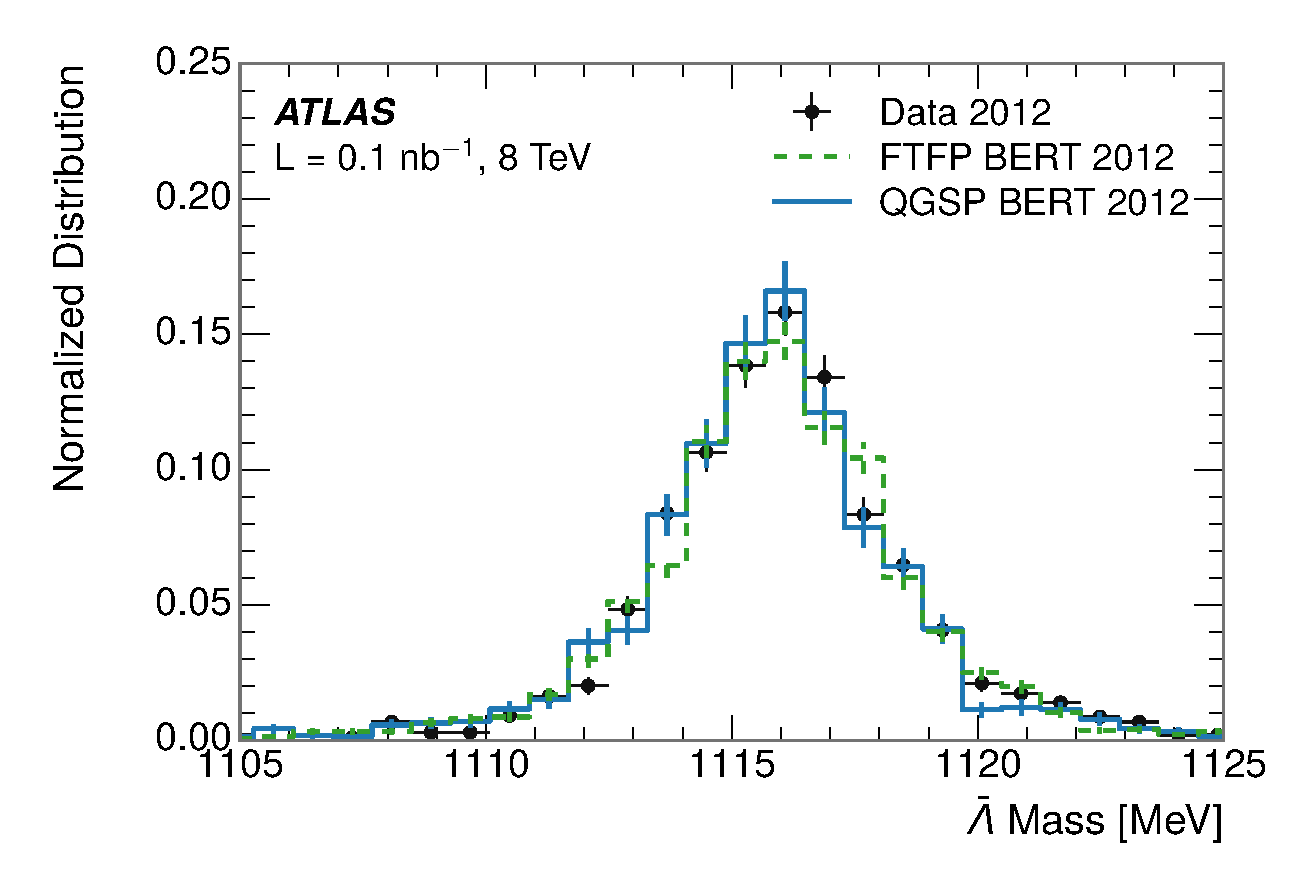
\includegraphics[width=\halffig]{figures/mass_lambdabar_eta01.pdf}
}
\caption{The reconstructed mass peaks of (a) \pKS, (b) \pL, and (c) \pLB candidates.}
\label{fig:identified_mass}
\end{figure}

The dominant backgrounds for the identified particle decays are nuclear interactions and combinatoric sources.
These are suppressed by the kinematic requirements on the tracks as well as an additional veto which removes candidates that are consistent with both a \pL or \pLB and a \pKS hypothesis, which is possible because of the different assumptions on particle mass in each case~\cite{PERF-2011-05}.
After these requirements, the backgrounds are found to be negligible compared to the statistical errors on these measurements. 

\subsection{Identified Response}
With these techniques the \ep distributions are extracted in data and simulation for each particle species and shown in Figure~\ref{fig:identified_eoverp}. 
These distributions are shown for a particular bin of $\Ea$ ($2.2 < \Ea / \GeV < 2.8$),  rather than p. 
$\Ea$ is the energy available to be deposited in the calorimeter: for pions $\Ea = \sqrt{p^2 + m_\pi^2}$, for protons $\Ea = \sqrt{p^2 + m_p^2} - m_p$, and for antiprotons $\Ea = \sqrt{p^2 + m_p^2} + m_p$.
In the pion case, the entire energy of the pion is deposited in the calorimeter, so \Ea is just the usual energy.
For protons, the proton remains after depositing its energy in the calorimeter, so its mass is not available and must be subtracted from \Ea.
And for antiprotons, the antiproton constituents annihilate with the quarks in the protons and neutrons of the calorimeter material, so it deposits its entire energy as well as an the additional energy from the annihilation; this extra energy is equal to the mass of the antiproton and is added to the available energy.
The features of the \ep distributions are similar to the inclusive case, with a peak around 0.5 at low momentum.
The zero fraction is not as pronounced as in the inclusive case.
There is a small negative tail from noise and a large fraction of tracks with zero energy from particles which do not reach the calorimeter.
The long positive tail is noticeably more pronounced for antiprotons because of the additional energy generated by the annihilation of the antiproton with the material of the detector, and the peak of the distribution is also increased for the same reason.
The simulation correctly captures these features, and the agreement between data and simulation is good to within the available statistical limitations.

\begin{figure}[h]
\centering
\subfloat[]{
  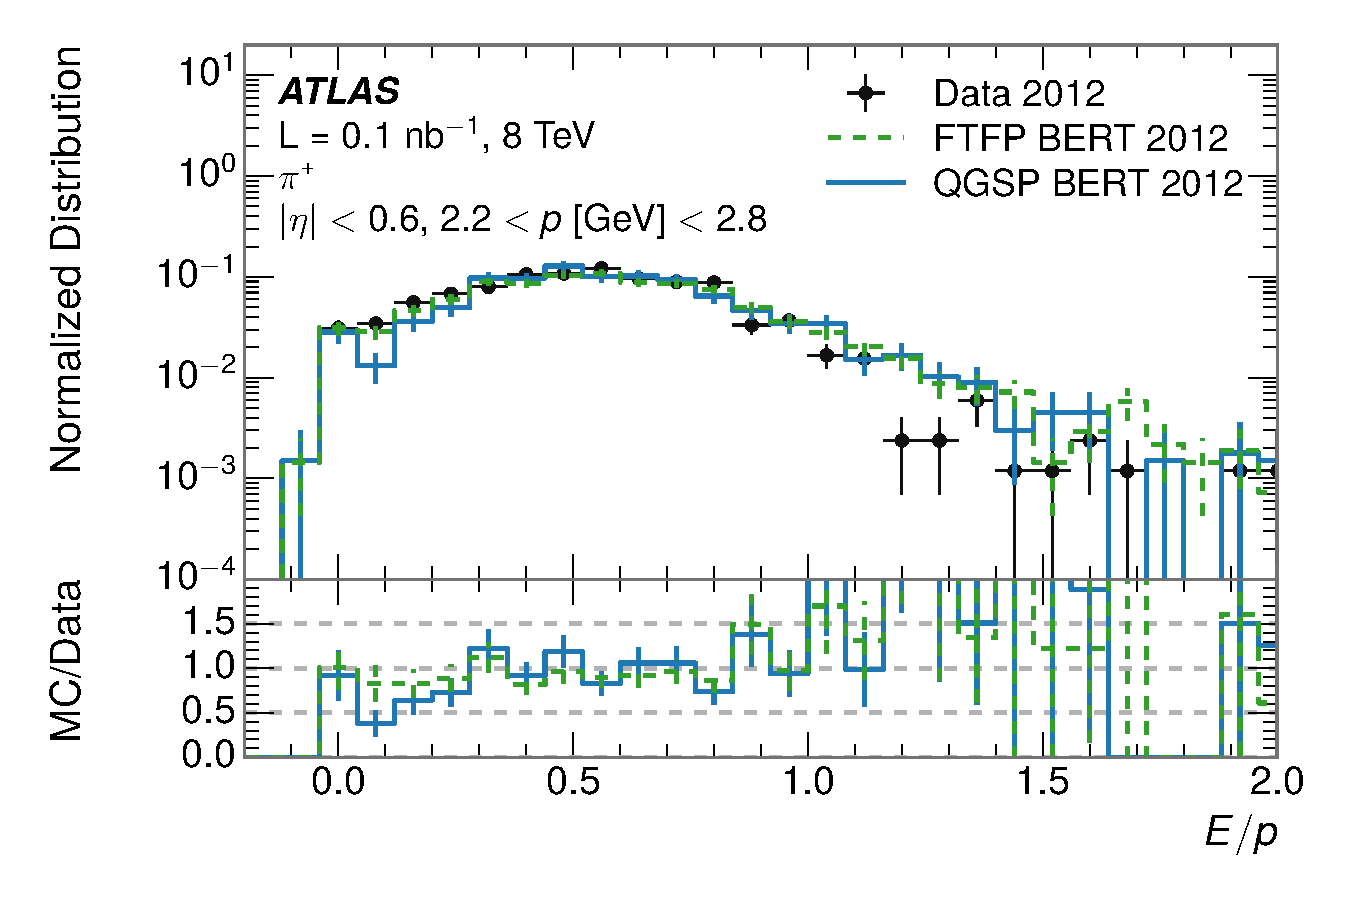
\includegraphics[width=\halffig]{figures/dvmc12r_eoverp_pip_eta01_p05.pdf}
}
~
\subfloat[]{
  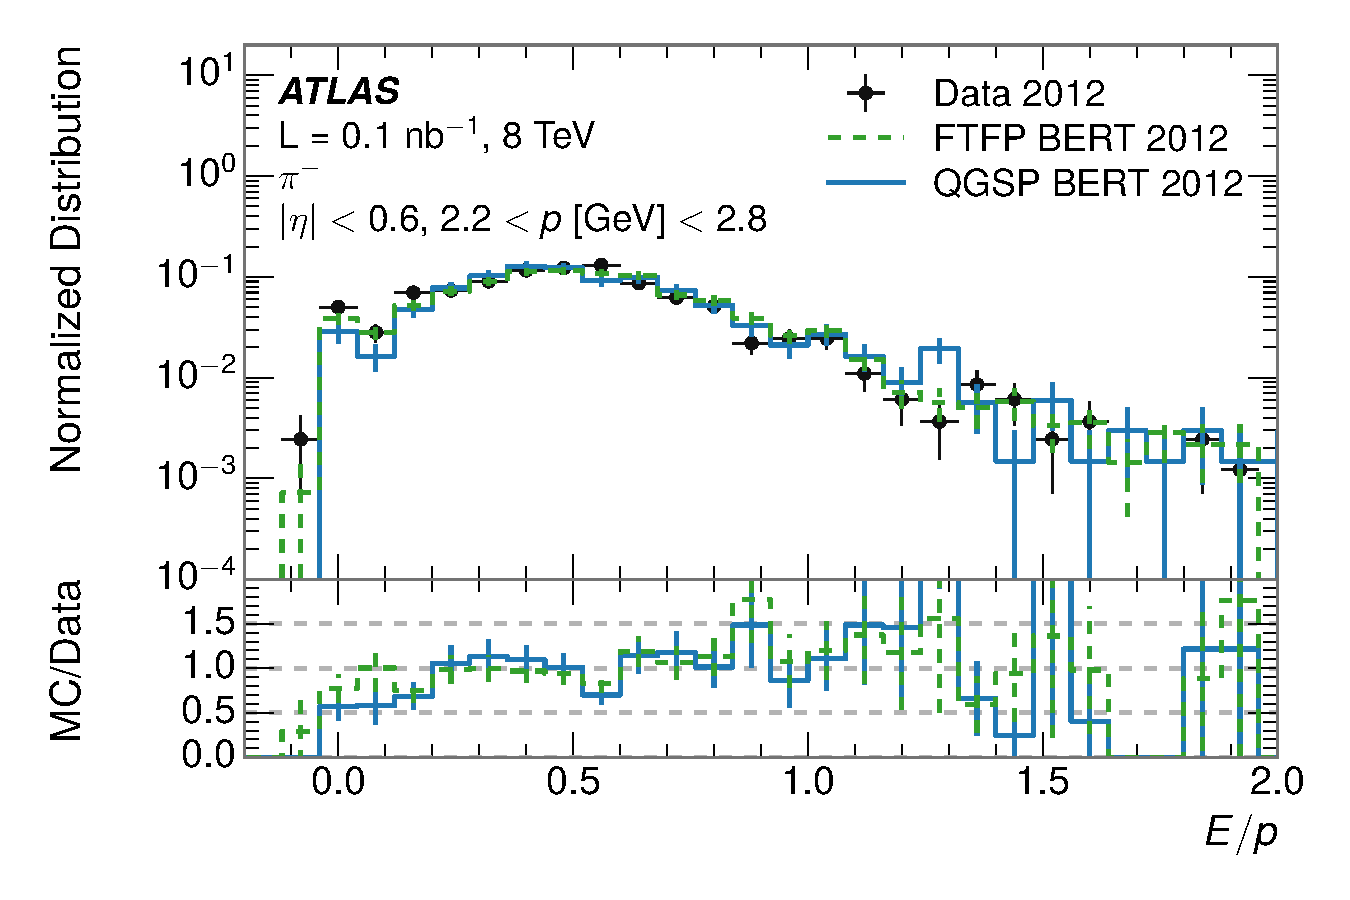
\includegraphics[width=\halffig]{figures/dvmc12r_eoverp_pim_eta01_p05.pdf}
}
\\
\subfloat[]{
  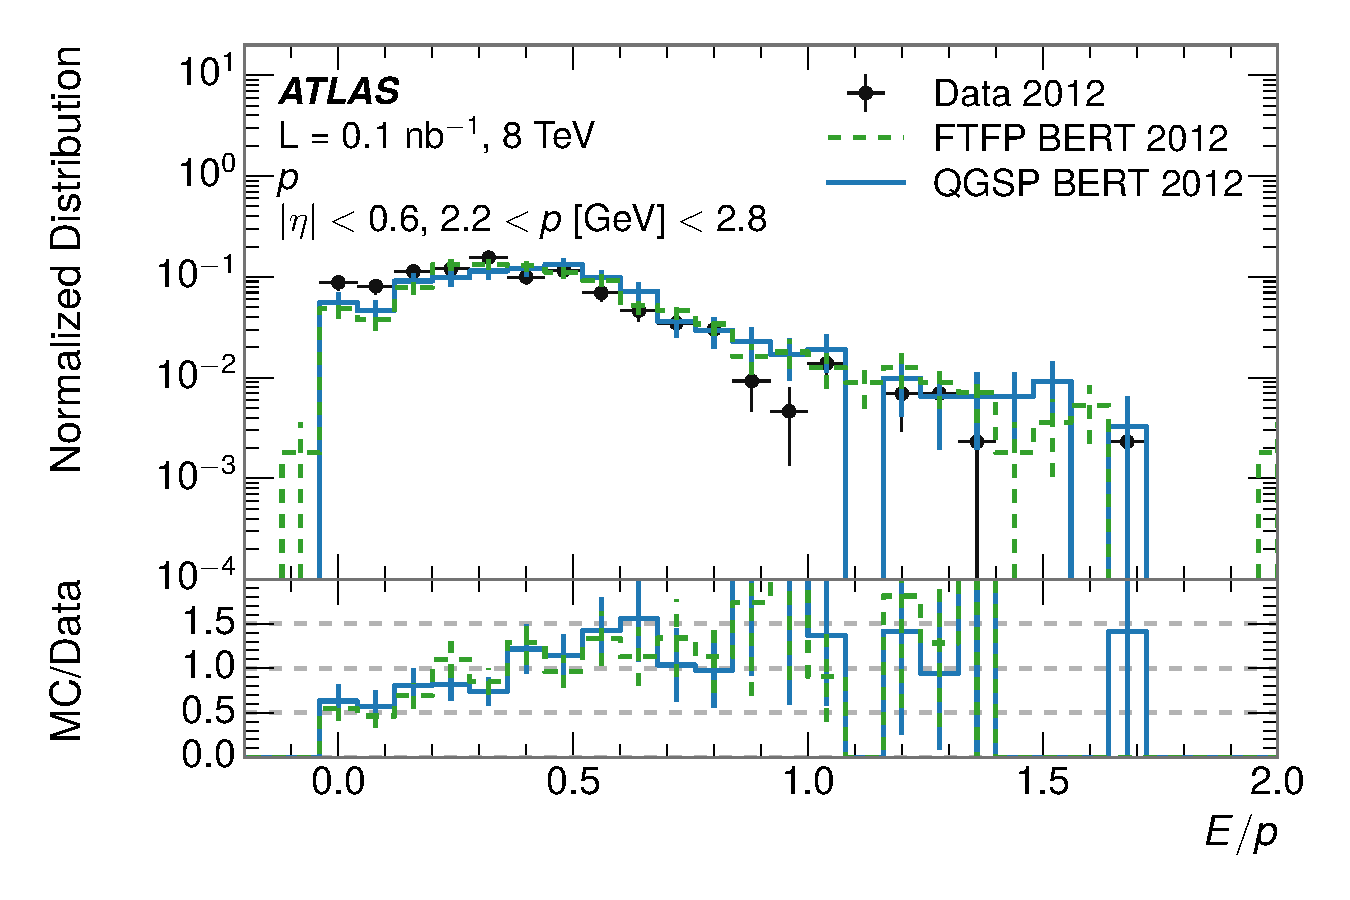
\includegraphics[width=\halffig]{figures/dvmc12r_eoverp_protonp_eta01_p05.pdf}
}
~
\subfloat[]{
  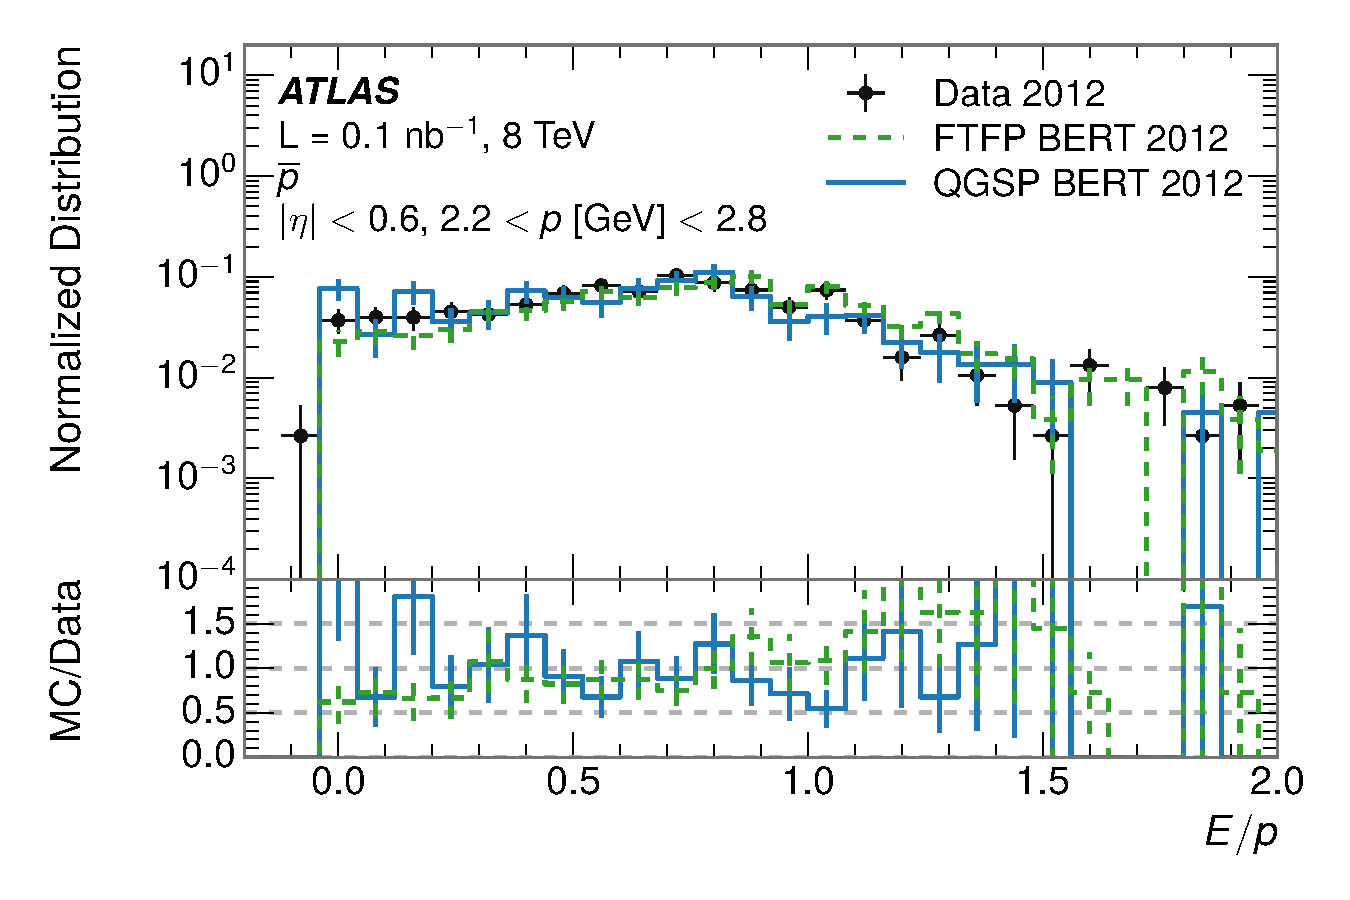
\includegraphics[width=\halffig]{figures/dvmc12r_eoverp_protonm_eta01_p05.pdf}
}
\caption{The \ep distribution for isolated (a) \pip, (b) \pim, (c) proton, and (d) anti-proton tracks.}
\label{fig:identified_eoverp}
\end{figure}

The zero fraction is further explored in Figure~\ref{fig:identified_zero_fraction} for pions and protons in data and simulation. 
The simulation consistently underestimates the zero fraction independent of particle species, which implies that this discrepancy is not caused by the model of a particular species but rather a feature common to all.
The zero fraction is larger for \pim than \pip, which is evident in both data and simulation.
However there is some suggestion that this increase in zero fraction leads to an even larger discrepancy in the modeling of \pim in simulation.

\begin{figure}[h]
\centering
\subfloat[]{
  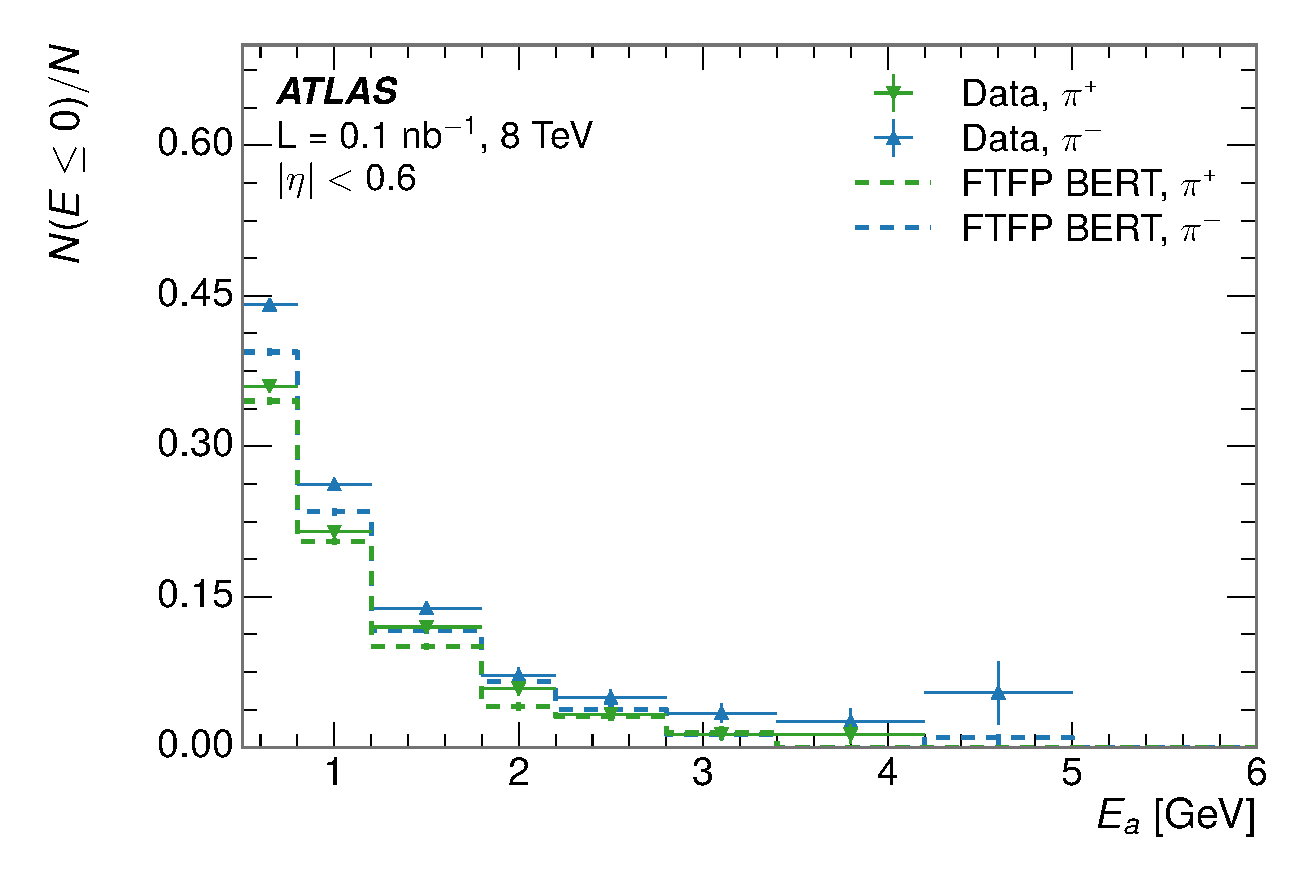
\includegraphics[width = \halffig]{figures/ep_zero_pions_eta01.pdf}
}
~
\subfloat[]{
  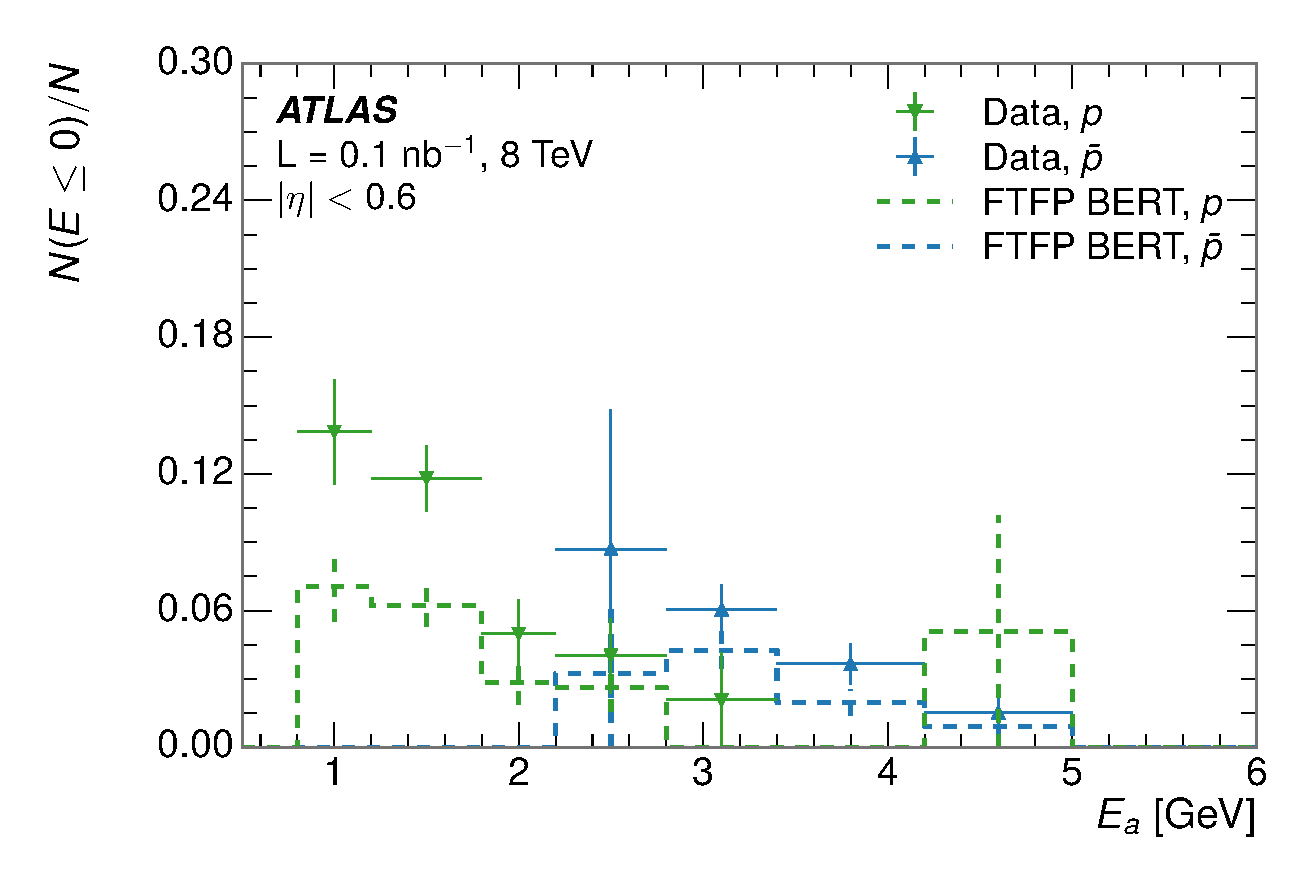
\includegraphics[width = \halffig]{figures/ep_zero_protons_eta01.pdf}
}
\caption{ The fraction of tracks with $E \leq 0$ for identified (a) \pip and \pim, and (b) proton and anti-proton tracks}
\label{fig:identified_zero_fraction}
\end{figure}

It is also interesting to compare the response between the different particle species.
One approach to do this is to measure the difference in \epav between two types, which has the advantage of removing the neutral background.
These differences are shown in various combinations in Figure~\ref{fig:identified_epdiff}. 
The response for \pip is greater on average than the response to \pim because of a charge-exchange effect which causes the production of additional neutral pions in the showers of \pip~\cite{particlebeam}. 
This effect becomes less significant as the \epav increases, and the difference approaches zero.
Both version of the simulation correctly model this trend.
The response for \pip is also greater on average than the response to \pP, because a large fraction of the energy of \pip hadrons is converted to an electromagnetic shower~\cite{physicsg,TileTB}. 
This effect is again reproduced by both simulations.
The \pAP response, however, is significantly higher than the response to \pim because of the annihilation of the antiproton, but the difference decreases at higher energies where the additional energy has less relative importance.
\FTFP models this effect more accurately than \QGSP because of their different descriptions of \pAP interactions with material.

\begin{figure}[htbp]
\centering
\subfloat[]{
  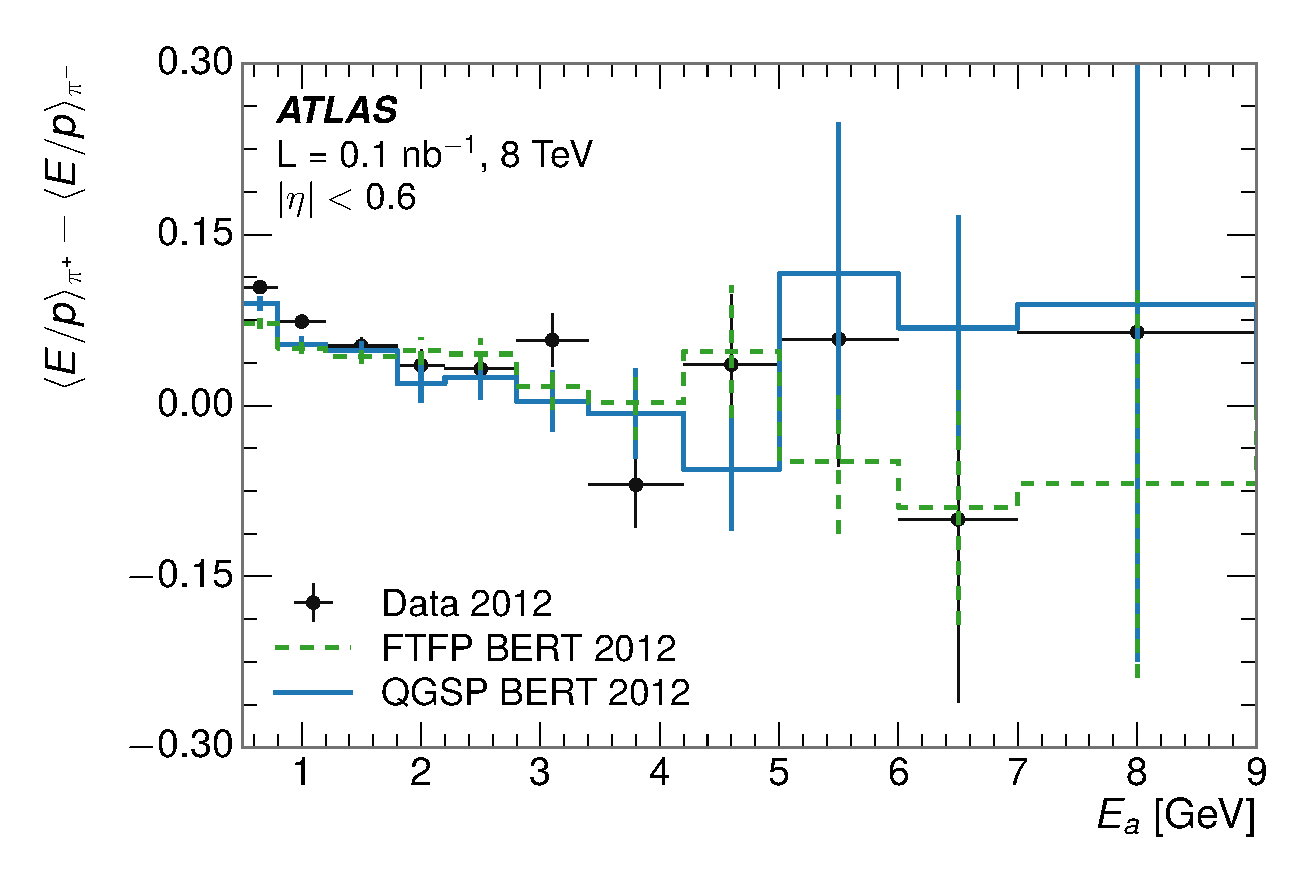
\includegraphics[width=\halffig]{figures/dvmc12r_epdiff_ea_pip_pim_eta01.pdf}
}
\\
\subfloat[]{
  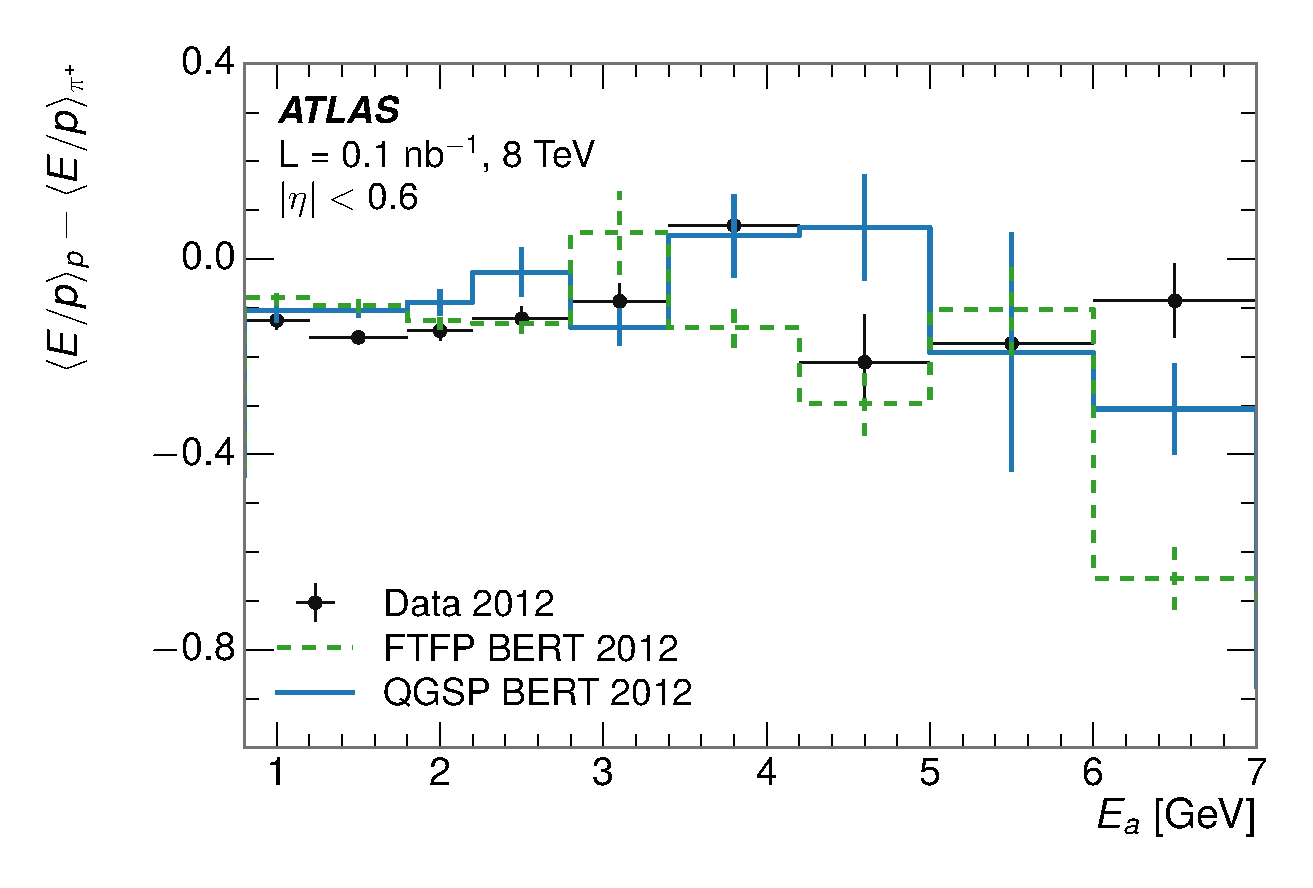
\includegraphics[width=\halffig]{figures/dvmc12r_epdiff_ea_protonp_pip_eta01.pdf}
}
~
\subfloat[]{
  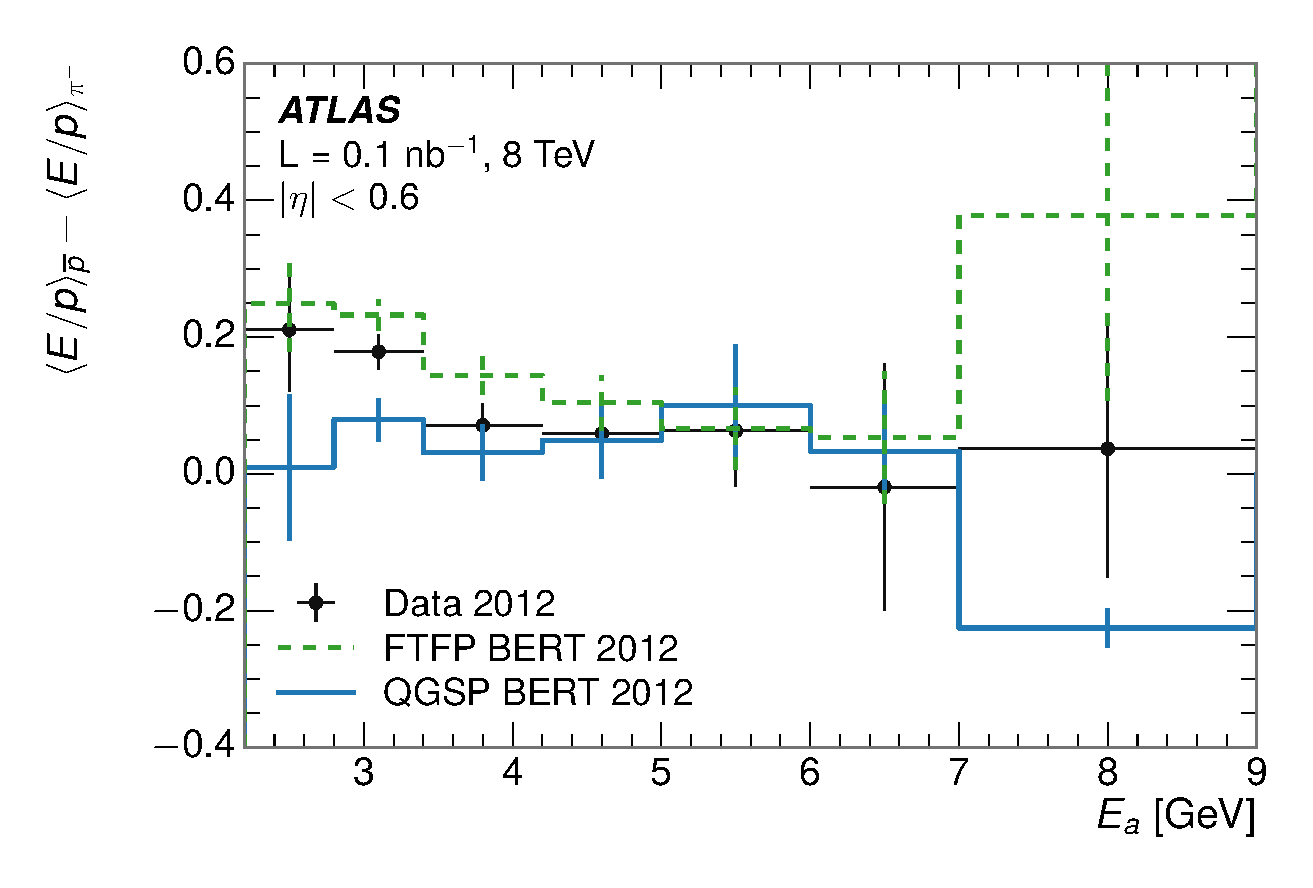
\includegraphics[width=\halffig]{figures/dvmc12r_epdiff_ea_protonm_pim_eta01.pdf}
}
\caption{ The difference in \epav between (a) \pip\ and \pim\, (b) \pP and \pip, and (c) \pAP and \pim.}
\label{fig:identified_epdiff}
\end{figure}

It is also possible to remove the neutral background from these response distributions using the same technique as in Section~\ref{sec:neutral_bg}. 
The technique is largely independent of the particle species and so can be directly applied to \epav for pions. 
The \epcor distributions for pions are shown in Figure~\ref{fig:identified_epcor}, which are very similar to the inclusive results.
The inclusive hadrons are comprised mostly of pions, so this similarity is not surprising.
It is also possible to see the small differences between \pip and \pim response here, where \epcor is higher on average for \pip.
The agreement between data and simulation is significantly worse for the \pim distributions than for the \pip, with a discrepancy greater than 10\% below 2-3 \GeV. 

\begin{figure}[h]
\centering
\subfloat[]{
  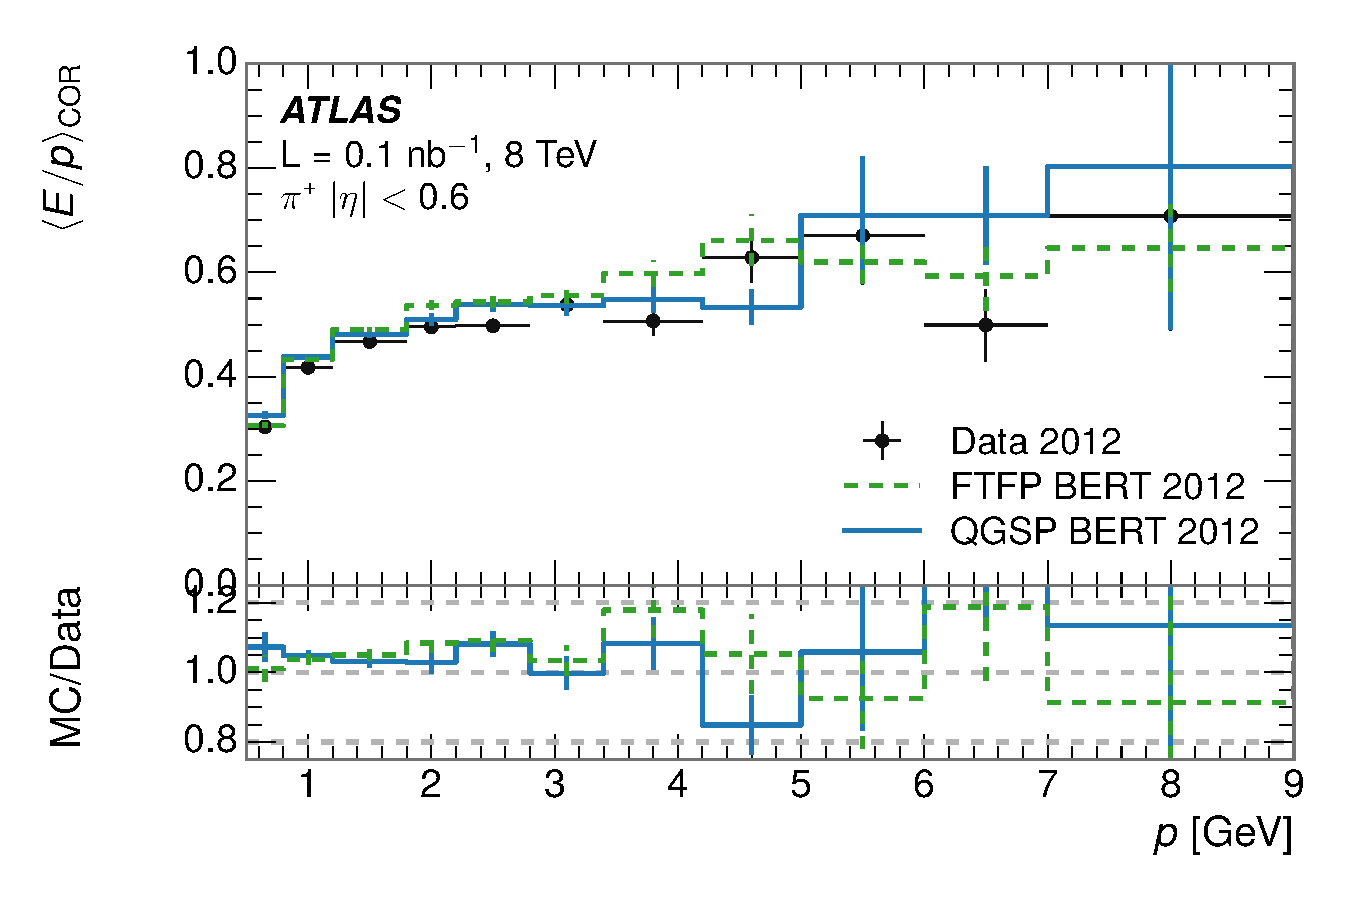
\includegraphics[width=\halffig]{figures/dvmc12r_epcor_p_pip_eta01.pdf}
}
\subfloat[]{
  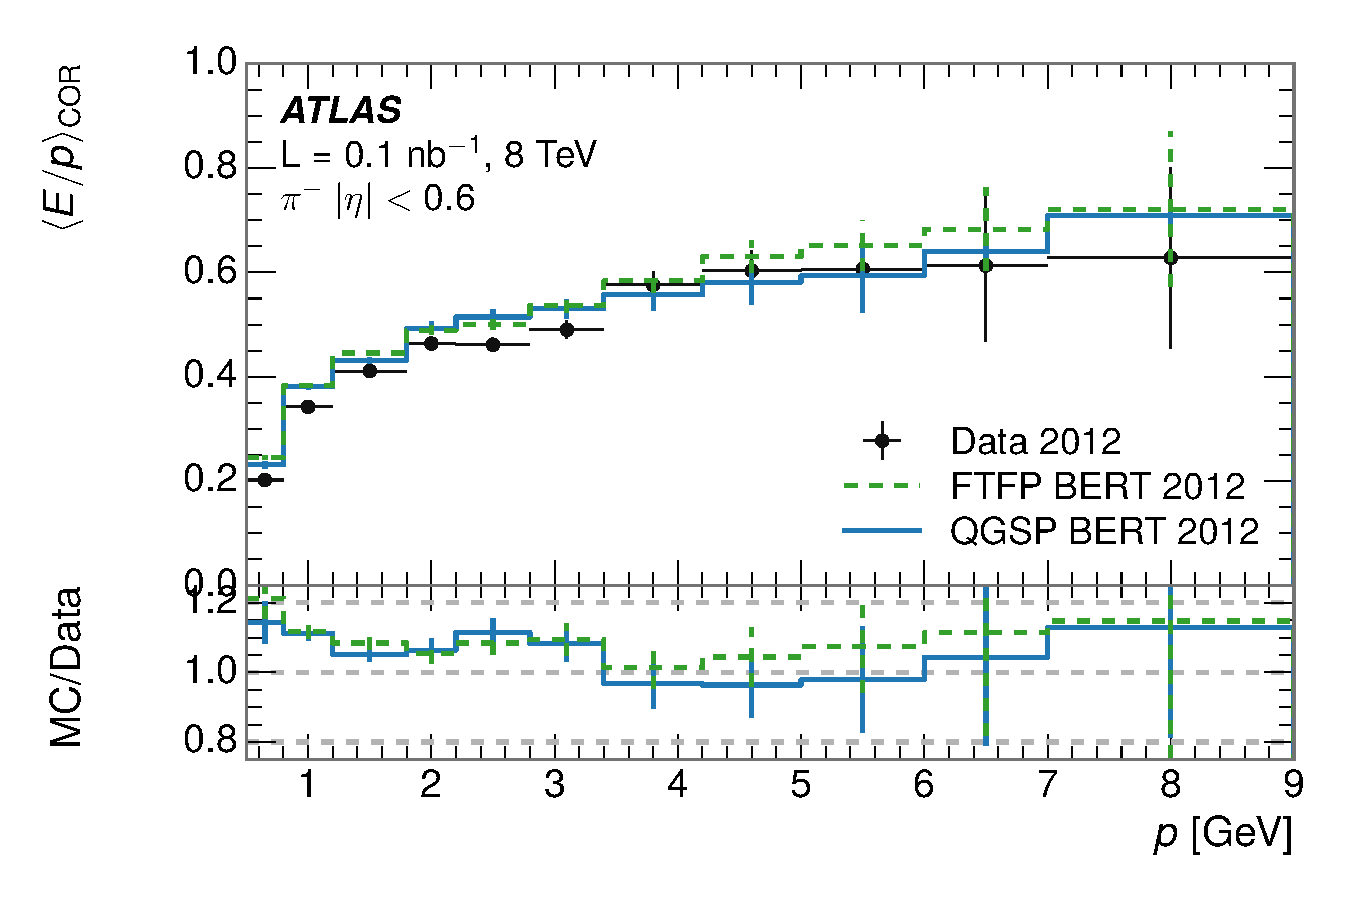
\includegraphics[width=\halffig]{figures/dvmc12r_epcor_p_pim_eta01.pdf}
}
\caption{\epcor as a function of track momentum for (a) \pip\ tracks and (b) \pim\ tracks.}
\label{fig:identified_epcor}
\end{figure}

\subsection{Additional Species in Simulation}

The techniques above provide a method to measure the response separately for only pions and protons. 
However the hadrons which forms jets include a number of additional species such as kaons and neutrons. 
The charged kaons are an important component of the inclusive charged hadron distribution, which is comprised of roughly 60-70\% pions, 15-20\% kaons, and 5-15\% protons~\cite{PERF-2015-05}.
These fractions vary depending on the production mechanism, and the ranges are indicative of the variations between different events.
These are difficult to measure in data at the ATLAS detector, as the particles which decay to kaons such as $\phi$ and $D$ mesons have shorter lifetimes and are comparatively rare. 
These properties make it impractical to identify a sufficient number of decays to make statistically meaningful measurements.
The simulation of these particles includes noticeable differences in response between species at low energies, which are shown in Figure~\ref{fig:simulated_response} for \FTFP.
The significant differences in response between protons and antiprotons below 1 \GeV are accounted for above in the definitions of \Ea. 

\begin{figure}[htbp]
\centering
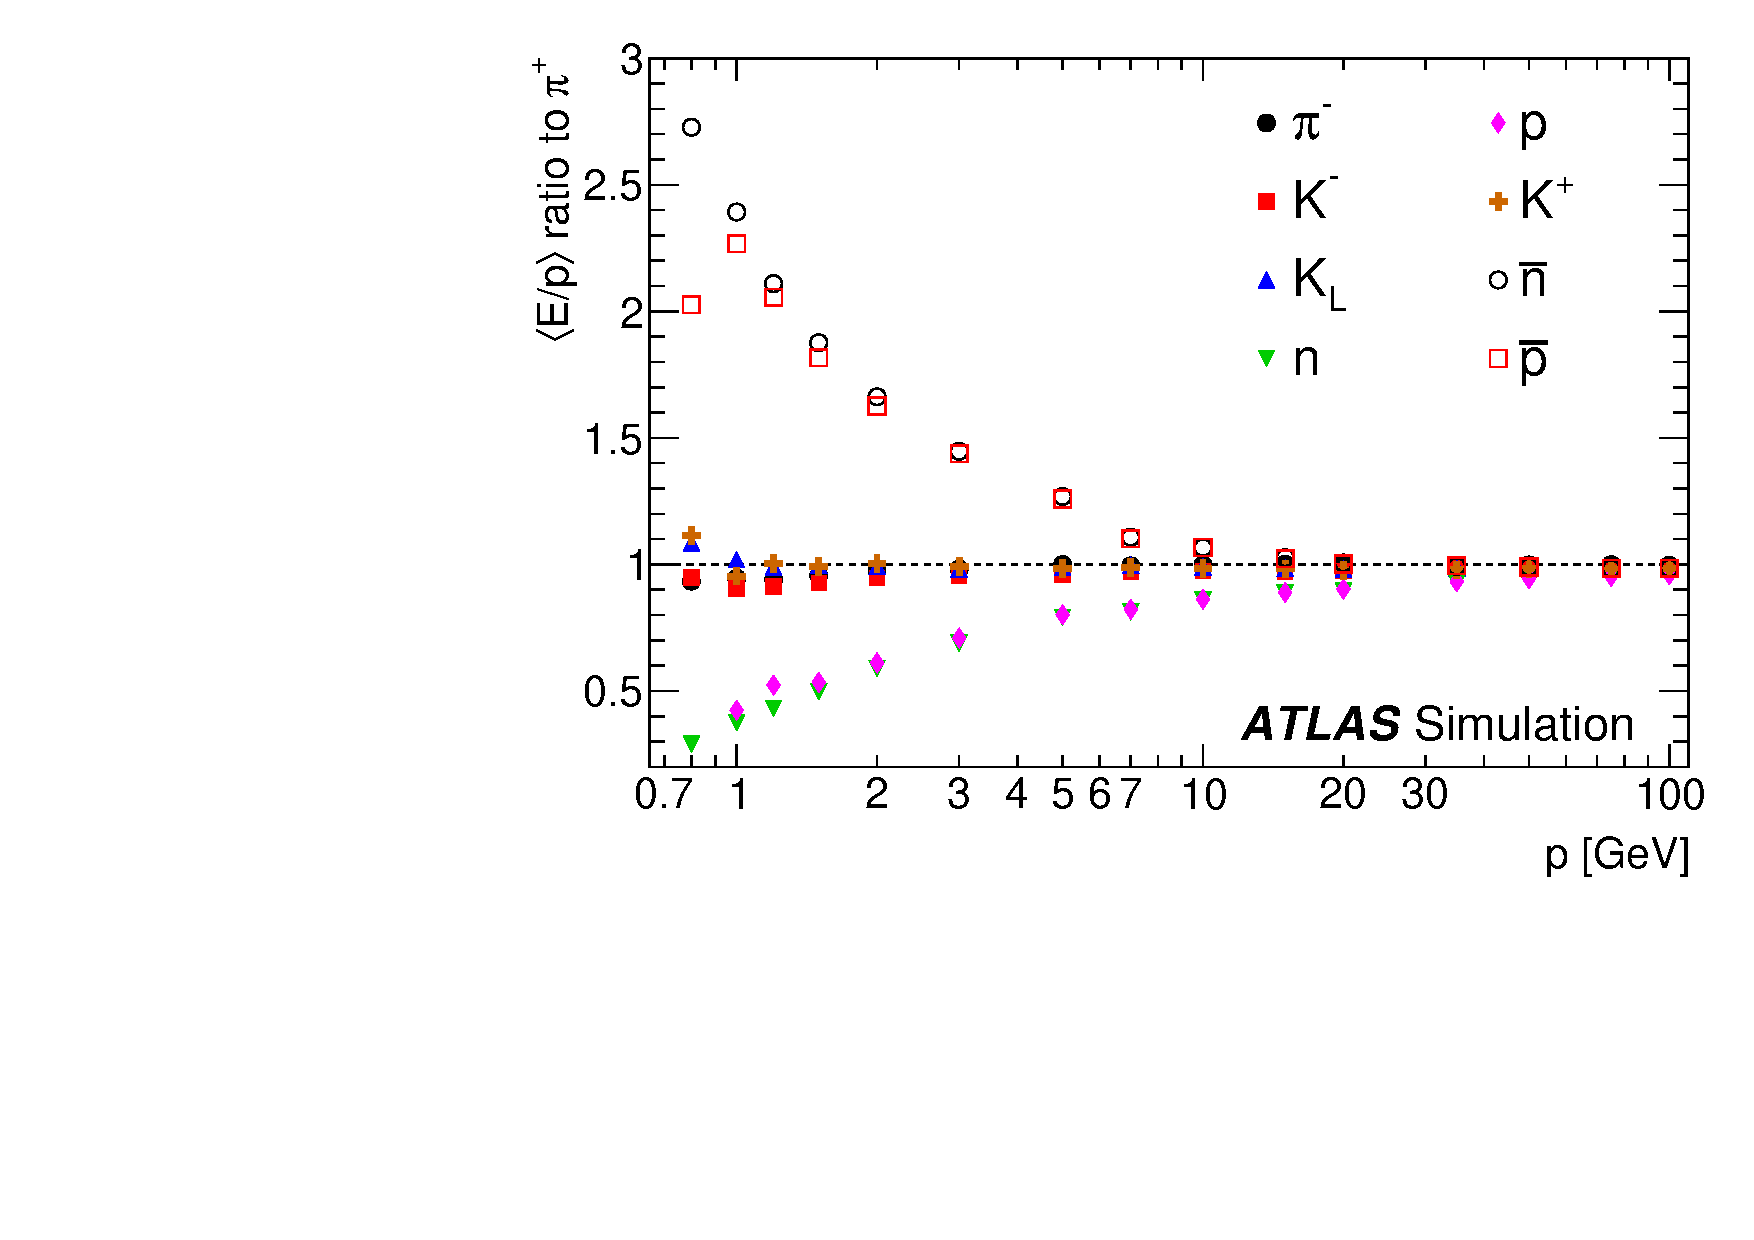
\includegraphics[width=\fullfig]{figures/simulated_response.pdf}
\caption{The ratio of the calorimeter response to single particles of various species to the calorimeter response to $\pi^+$ with the physics list \texttt{FTFP\_BERT}.}
\label{fig:simulated_response}
\end{figure}

% ----------------------------------------

\section{Summary}

These various measurements of calorimeter response shown above for data and simulation illuminate the accuracy of the simulation of hadronic interactions at the ATLAS detector. 
The results were obtained using 2010 and 2012 data at 7 and 8 \TeV, but reflect the most current understanding of the detector alignment and geometry.
A number of measurements focusing on a comparison between protons and antiprotons suggest that \FTFP models those interaction more accurately than \QGSP.
These measurements, among others, were the motivation to switch the default \texttt{Geant4} simulation from \QGSP to \FTFP for all ATLAS samples. 

Even with these updates, there are a number of approximately 5\% discrepancies in response between the data and simulation.
The differences result mostly from a difference in the modeling of the zero fraction, which is most significant at low energies.
The difference in response without the zero fraction are primarily in the electromagnetic calorimeter, while the modeling of the hadronic calorimeter is accurate.
At higher momenta the simulation of hadronic interactions is very consistent with data. 
Chapter~\ref{ch:jes} discusses how to use these observed differences to constrain the jet energy scale and its associated uncertainties.
